% CREATED BY DAVID FRISK, 2017

% IMPORT SETTINGS
\documentclass[12pt,a4paper,twoside,openright]{article}
% CREATED BY DAVID FRISK, 2016

% to use subfigures
\usepackage{subcaption}

% BASIC SETTINGS
\usepackage{grffile}
\usepackage{moreverb}								% List settings
\usepackage{textcomp}								% Fonts, symbols etc.
\usepackage{lmodern}								% Latin modern font
\usepackage{helvet}									% Enables font switching
\usepackage[T1]{fontenc}							% Output settings
\usepackage[english]{babel}							% Language settings
\usepackage[utf8]{inputenc}							% Input settings
\usepackage{amsmath}								% Mathematical expressions (American mathematical society)
\usepackage{amssymb}								% Mathematical symbols (American mathematical society)
\usepackage{graphicx}								% Figures
%\usepackage{subfig}									% Enables subfigures
\usepackage{listings}								% Enables source code listings
\usepackage{chemfig}								% Chemical structures
\usepackage[top=3cm, bottom=3cm,
			inner=3cm, outer=3cm]{geometry}			% Page margin lengths			
\usepackage{eso-pic}								% Create cover page background
\newcommand{\backgroundpic}[3]{
	\put(#1,#2){
	\parbox[b][\paperheight]{\paperwidth}{
	\centering
	\includegraphics[width=\paperwidth,height=\paperheight,keepaspectratio]{#3}}}}
\usepackage{float} 									% Enables object position enforcement using [H]
%\usepackage{parskip}								% Enables vertical spaces correctly 

% For using gray lines in table
\usepackage{colortbl}



% OPTIONAL SETTINGS (DELETE OR COMMENT TO SUPRESS)

% Disable automatic indentation (equal to using \noindent)
%\setlength{\parindent}{0cm}                         


% Caption settings (aligned left with bold name)
\usepackage[labelfont=bf, textfont=normal,
			justification=justified,
			singlelinecheck=false]{caption} 		

		  	
% Activate clickable links in table of contents  	
\usepackage{hyperref}								
\hypersetup{colorlinks, citecolor=black,
   		 	filecolor=black, linkcolor=black,
    		urlcolor=black}


% Define the number of section levels to be included in the t.o.c. and numbered	(3 is default)	
\setcounter{tocdepth}{2}							
\setcounter{secnumdepth}{3}	


% Chapter title settings
%\usepackage{titlesec}		
%\titleformat{\chapter}[display]
%  {\Huge\bfseries\filcenter}
%  {{\fontsize{50pt}{1em}\vspace{-4.2ex}\selectfont \textnormal{\thechapter}}}{1ex}{}[]


% Header and footer settings (Select TWOSIDE or ONESIDE layout below)
\usepackage{fancyhdr}								
\pagestyle{fancy}  



% Select one-sided (1) or two-sided (2) page numbering
\def\layout{2}	% Choose 1 for one-sided or 2 for two-sided layout
% Conditional expression based on the layout choice
\ifnum\layout=2	% Two-sided
    \fancyhf{}			 						
	\fancyhead[LE,RO]{\nouppercase{ \leftmark}}
	\fancyfoot[LE,RO]{\thepage}
	\fancypagestyle{plain}{			% Redefine the plain page style
	\fancyhf{}
	\renewcommand{\headrulewidth}{0pt} 		
	\fancyfoot[LE,RO]{\thepage}}	
\else			% One-sided  	
  	\fancyhf{}					
	\fancyhead[C]{\nouppercase{ \leftmark}}
	\fancyfoot[C]{\thepage}
\fi


% Enable To-do notes
\usepackage[textsize=tiny]{todonotes}   % Include the option "disable" to hide all notes
\setlength{\marginparwidth}{2.5cm} 


% Supress warning from Texmaker about headheight
\setlength{\headheight}{15pt}		

\newcommand{\grayline}[1]{
    \arrayrulecolor{gray}\cline{#1}\arrayrulecolor{black}
}

%\setcounter{tocdepth}{0}
\begin{document} 

% COVER PAGE, TITLE PAGE AND IMPRINT PAGE
\pagenumbering{roman}			% Roman numbering (starting with i (one)) until first main chapter
% CREATED BY DAVID FRISK, 2016

% COVER PAGE
\begin{titlepage}
\newgeometry{top=3cm, bottom=3cm,
			left=2.25 cm, right=2.25cm}	% Temporarily change margins		
			
% Cover page background 
\AddToShipoutPicture*{\backgroundpic{-4}{56.7}{include/figure/auxiliary/frontpage_eng.pdf}}
\addtolength{\voffset}{2cm}

% Cover picture (replace with your own or delete)		
\begin{figure}[H]
\centering
\vspace{1cm}	% Adjust vertical spacing here
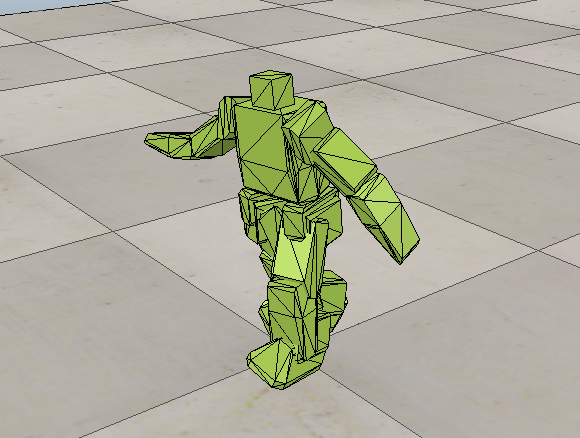
\includegraphics[width=0.9\linewidth]{include/figure/auxiliary/frontpage.png}
\end{figure}

% Cover text
\mbox{}
\vfill
\renewcommand{\familydefault}{\sfdefault} \normalfont % Set cover page font
\textbf{{\Huge EVOLVING A HUMANOID BEHAVIOUR  	\\[0.2cm] 
				IN A CPG ROBOT}} 	\\[0.5cm]
%{\Large A Subtitle that can be Very Much Longer if Necessary}\\[0.5cm]
Humanoid Robotics TIF160 \setlength{\parskip}{1.0cm}\vspace{0.25cm}\\
{\large NILS CARLSSON\\ JOHAN LARSSON HÖRKÉN \\ FREDDIE OGEMARK} \setlength{\parskip}{2.9cm}

\renewcommand{\familydefault}{\rmdefault} \normalfont % Reset standard font
\end{titlepage}


% BACK OF COVER PAGE (BLANK PAGE)
%\newpage
%\restoregeometry
%\thispagestyle{empty}
%\mbox{}


% TITLE PAGE
%\newpage
%\thispagestyle{empty}
%\begin{center}
%	\textsc{\large Master's thesis 2017:NN}\\[4cm]		% Report number given by department 
%	\textbf{\Large An Informative Headline describing\\ the Content of the Report} \\[1cm]
%	{\large A Subtitle that can be Very Much Longer if Necessary}\\[1cm]
%	{\large NAME FAMILYNAME}
	
%	\vfill	
	% Logotype on titlepage	
%	\begin{figure}[H]
%	\centering
	% Remove the following line to remove the titlepage logotype
%	
\includegraphics[width=0.2\pdfpagewidth]{figure/auxiliary/logo_eng.pdf} \\	
%	\end{figure}	\vspace{5mm}	
	
%	Department of Some Subject or Technology \\
%	\emph{Division of Division name}\\
%	Name of research group (if applicable)\\
%	\textsc{Chalmers University of Technology} \\
%	Gothenburg, Sweden 2017 \\
%\end{center}


% IMPRINT PAGE (BACK OF TITLE PAGE)
%\newpage
%\thispagestyle{plain}
%\vspace*{4.5cm}
%An Informative Headline describing the Content of the Report\\
%A Subtitle that can be Very Much Longer if Necessary\\
%NAME FAMILYNAME \setlength{\parskip}{1cm}

%\copyright ~ NAME FAMILYNAME, 2017. \setlength{\parskip}{1cm}

%Supervisor: Name, Company or Department\\
%Examiner: Name, Department \setlength{\parskip}{1cm}

%Master's Thesis 2017:NN\\	% Report number given by department 
%Department of Some Subject or Technology\\
%Division of Division name\\
%Name of research group (if applicable)\\
%Chalmers University of Technology\\
%SE-412 96 Gothenburg\\
%Telephone +46 31 772 1000 \setlength{\parskip}{0.5cm}

%\vfill
% Caption for cover page figure if used, possibly with reference to further information in the report
%Cover: Wind visualization constructed in Matlab showing a surface of constant wind speed along with streamlines of the flow. \setlength{\parskip}{0.5cm}

%Typeset in \LaTeX \\
%Printed by [Name of printing company]\\
%Gothenburg, Sweden 2017



% ABSTRACT
\newpage
\thispagestyle{plain}			% Supress header 
\setlength{\parskip}{0pt plus 1.0pt}
\section*{Abstract}
A walking cycle for a humanoid robot can be generated through means of reinforced learning algorithms, such as a genetic algorithm. Using data captured from human movements could potentially lead to a faster convergence of the algortihm along with more stable results. A simulation was set up consisting of a CPG network connected to a genetic algorithm, along with a 3D simulation of a humanoid robot. Accelerometer data from a human walking cycle was inserted as a starting point for the algorithm in order to see if the speed and accuracy of the simulation was improved. The results from the simulation was connected to a physical humanoid robot to evaluate the generated movement pattern. Although the results were found to be unstable, the method does show potential for improvement and refinement.
% KEYWORDS (MAXIMUM 10 WORDS)
\vfill
Keywords: CPG, Bioloid, Genetic Algorithm, V-REP, Walk Cycle, Humanoid Robot, Reinforced Learning.
\newpage				% Create empty back of side
\thispagestyle{empty}
\mbox{}

% ACKNOWLEDGEMENTS
%\newpage
%\input{include/frontmatter/Acknowledgements}


% TABLE OF CONTENTS
\tableofcontents

\newpage

% OTHER FRONTMATTER
% List of figures (add to table of contents)
%\cleardoublepage
%\addcontentsline{toc}{chapter}{\listfigurename} 
%\listoffigures
% List of tables (add to table of contents)
%\cleardoublepage
%\addcontentsline{toc}{chapter}{\listtablename}  
%\listoftables


% START OF MAIN DOCUMENT
%\cleardoublepage
\setcounter{page}{1}
\pagenumbering{arabic}			% Arabic numbering starting from 1 (one)
\setlength{\parskip}{0pt plus 1pt}

% INTRODUCTION
\newpage
% CREATED BY DAVID FRISK, 2016
\section{Introduction}
The field of humanoid robotics is a fast growing field of research and development wherein humanoid robots are becoming more and more advanced. There are different ways for a humanoid robot to interact with the world. Walking is one of the rudimentary characteristics of human movement, achieving a bipedal walking gait allows a robot to perform more complex tasks in a world adapted for humans, but constructing a robust walking gait is not trivial. There has been a lot of research and development using Central Pattern Generators (CPGs) to construct a walking gait using Genetic Algorithms (GA) as reinforced learning method. These algorithms are known to take very long to evolve a robust walking cycle. In most projects the GA starts with a random seed, which is one of the reasons for the long time needed to evolve a good walking cylce. 


\subsection{Purpose}
The aim of this project is to investigate if using data gathered from a human walking cycle as the seed in the GA of a CPG will make the GA evolve faster and give a better walking cycle compared to using a random seed and letting it evolve from scratch. The robot used as the target platform for the movement cycle is the Bioloid robot \cite{bioloid}, shown in Figure \ref{fig:bioloid}.

\begin{figure}[htbp]
    \centering
    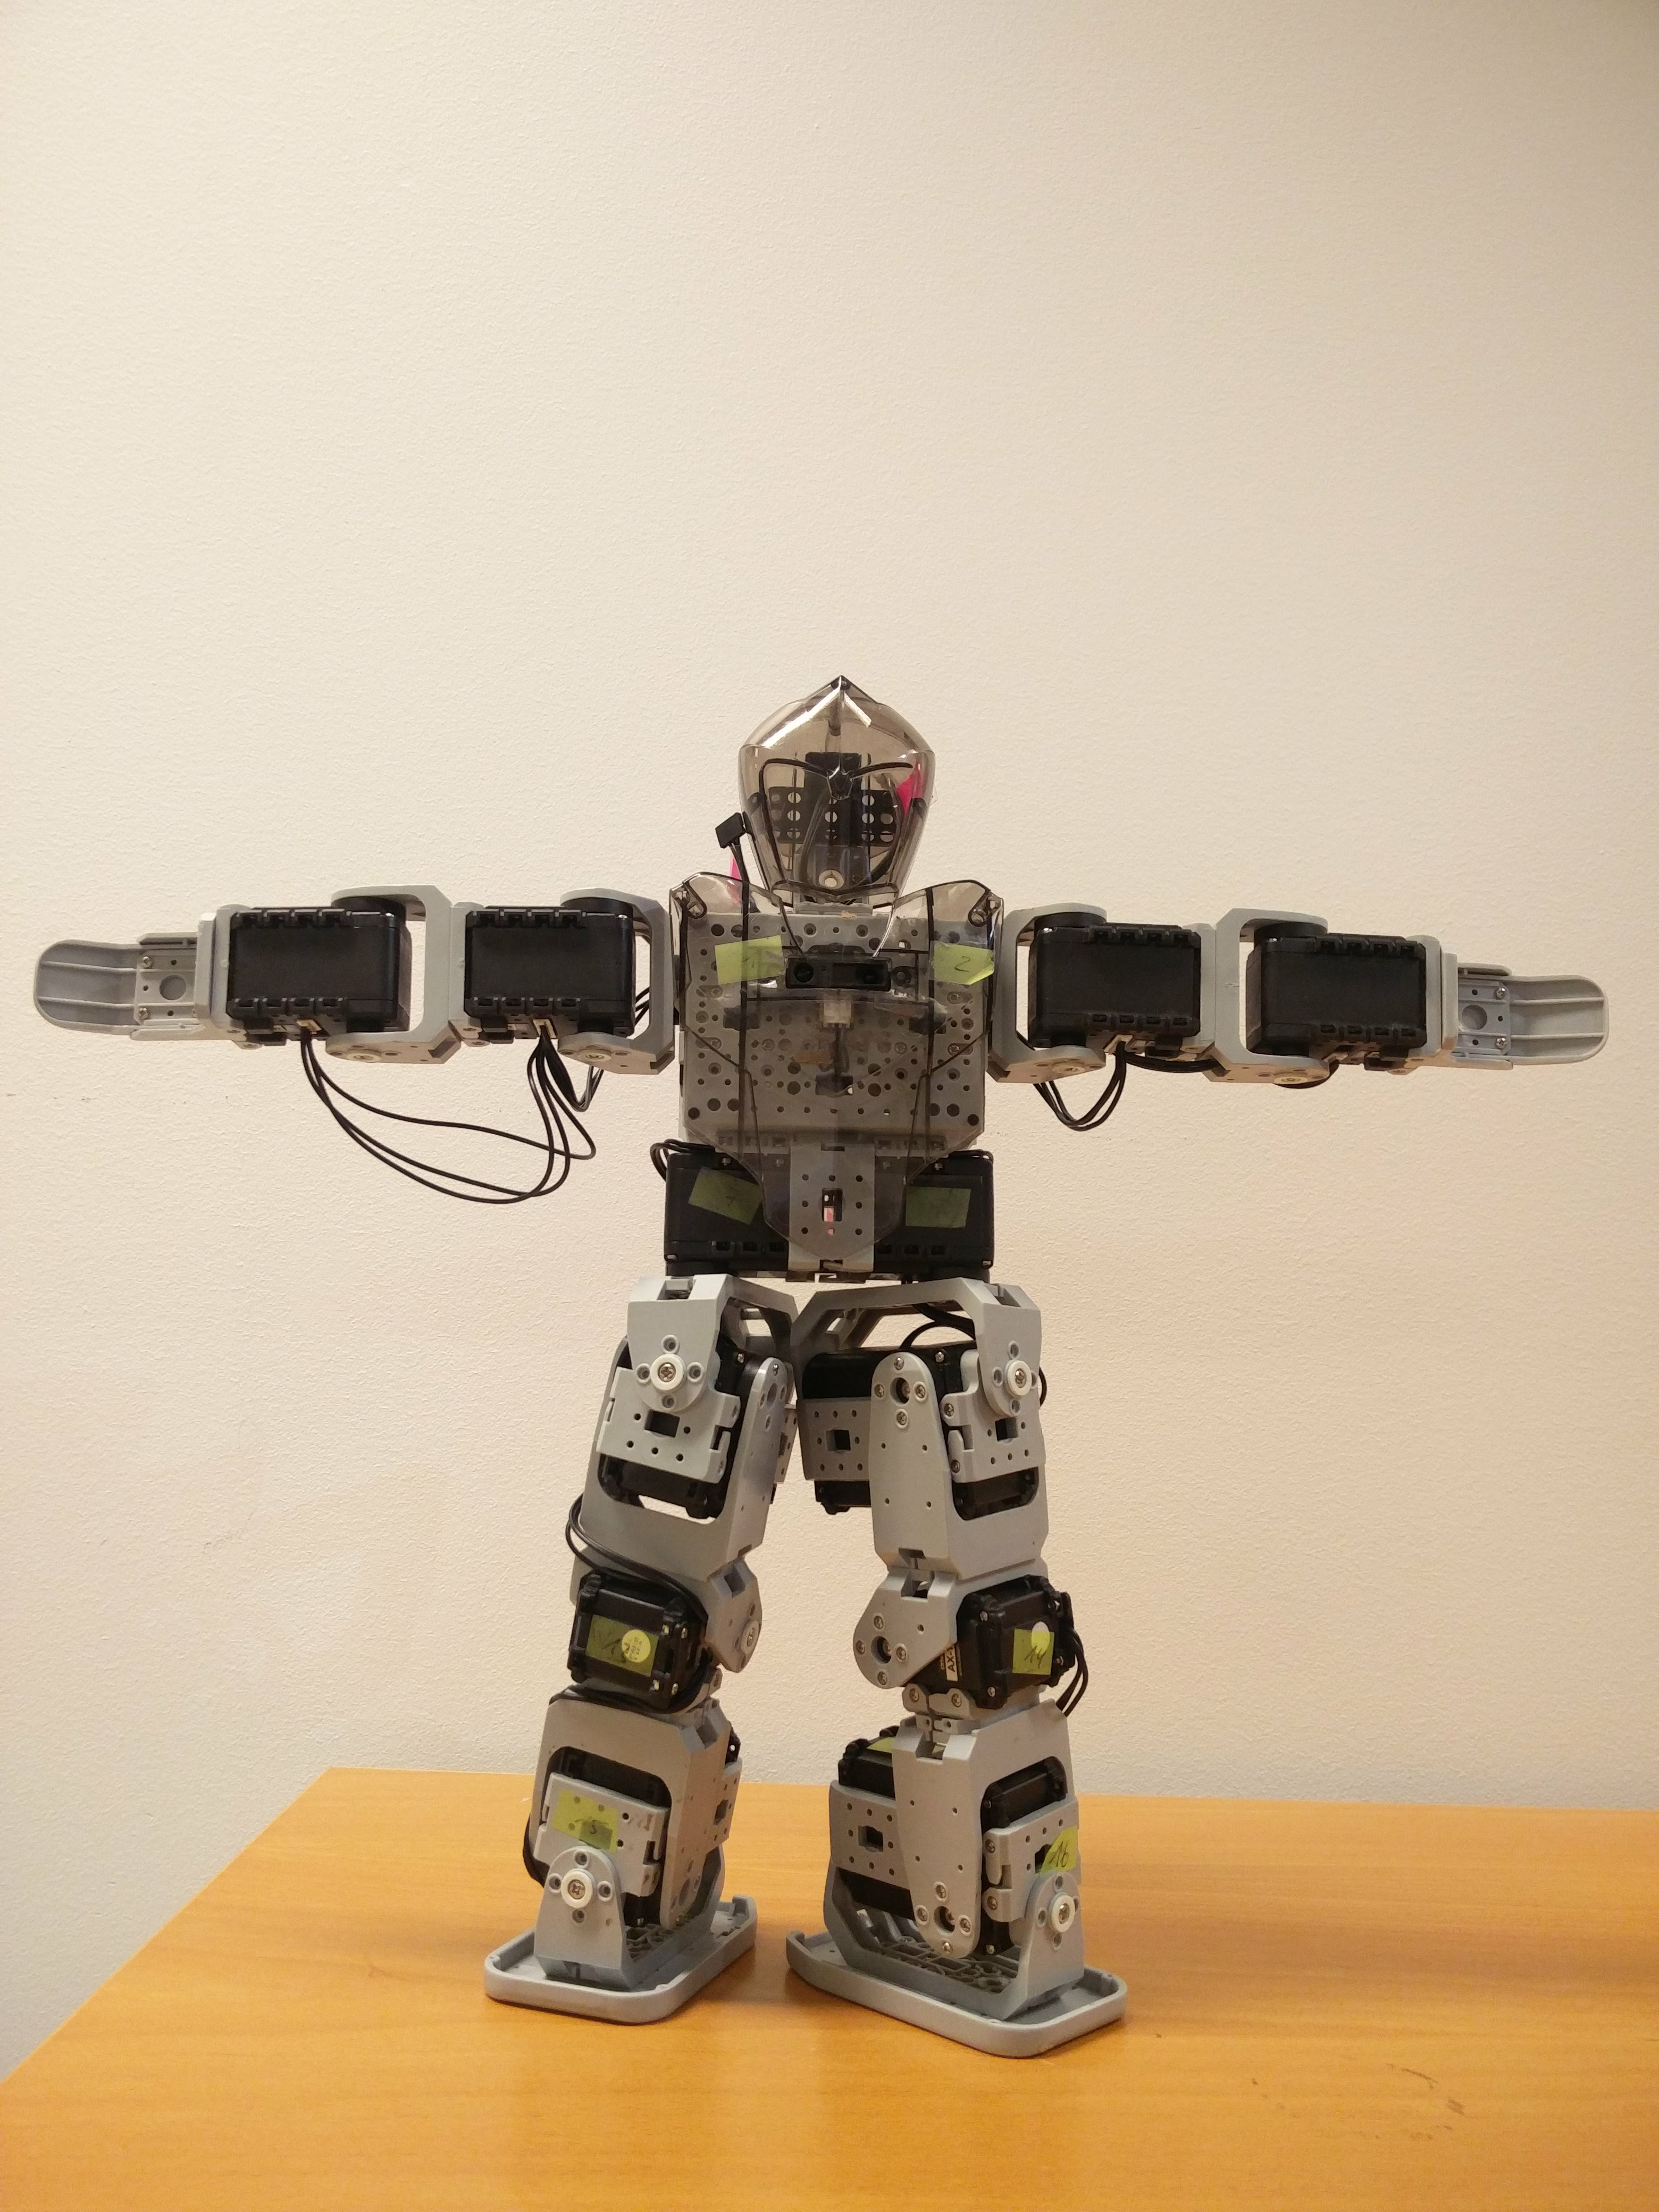
\includegraphics[width=0.35\textwidth]{include/figure/robot.jpg}
    \caption{The Bioloid robot used throughout this project.}
    \label{fig:bioloid}
\end{figure}

% THEORY
\newpage
% CREATED BY DAVID FRISK, 2016
\section{Theory}
In the following the section the underlying theory of the models used in the project are introduced and explained, along with relevant background and examples. 

\subsection{CPG Model}

\subsubsection{Mathematical Model of Physical Behaviour}
%CPG is a mathematical model of human/animal behaviour. Limit cycle, standing wave. Robust, can handle disturbance. (Model different different joints as CPG. Model different DoF as CPG.)

Biological behaviour in mammals, such as walking or swimming, are usually repetative and oscillatory creating energy efficient movements. This can be seen in Figure \ref{fig:walkingCycle}, which shows the walking cycle of a human, measured as the acceleration in Z-direction whilst walking. Due to the rhytmic patterns in the behaviour, it is possible to construct a mathematical model to mimic this type of behaviour. 

\begin{figure}[htbp]
    \centering
    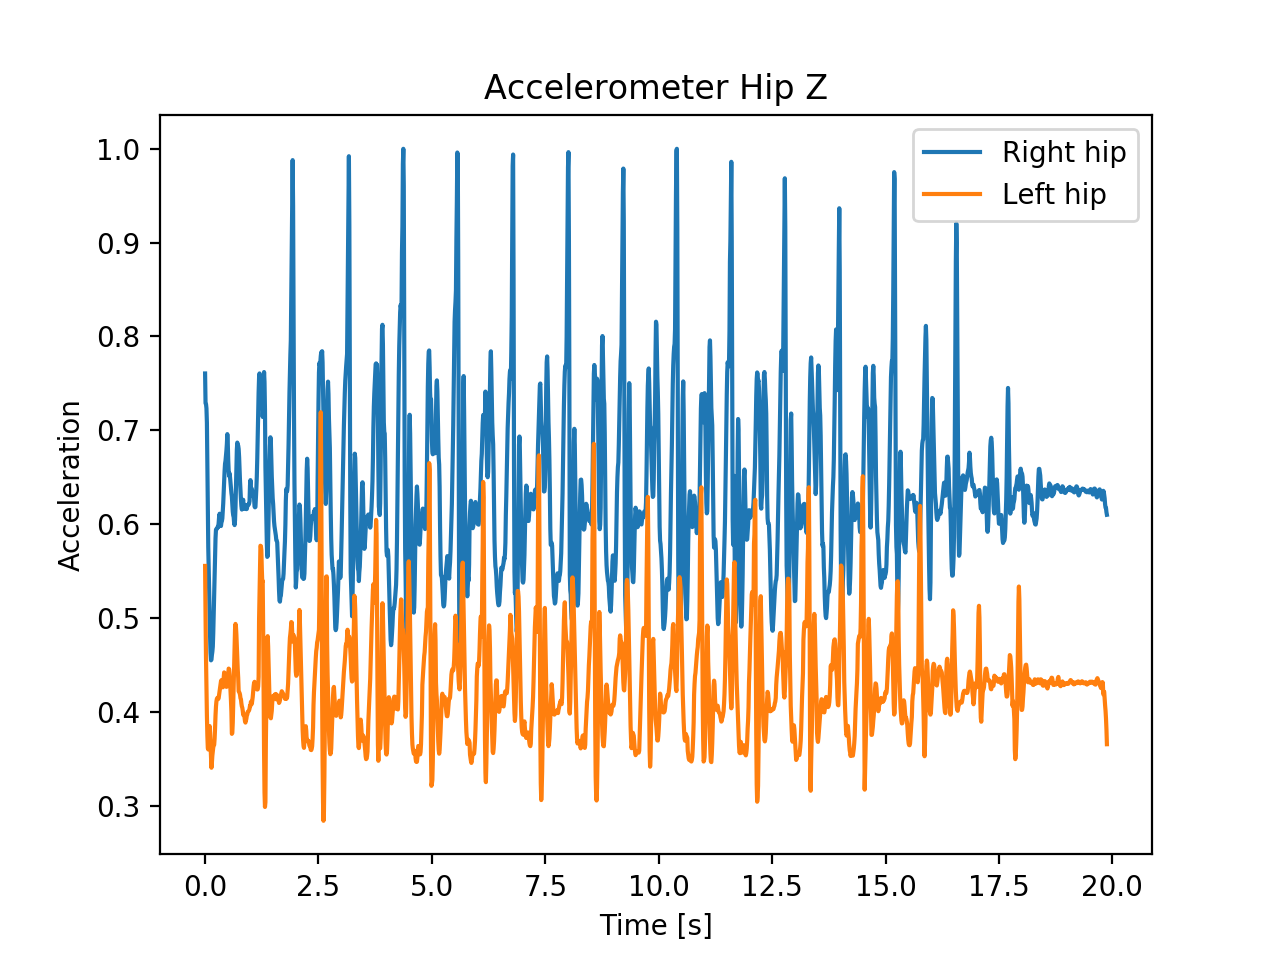
\includegraphics[width=.75\textwidth]{include/figure/reference_right_hip_z.png}
    \caption{Walking cycle of a human. Where \textit{Z} is the horizontal direction of the reference system.}
    \label{fig:walkingCycle}
\end{figure}

A Central Pattern Generator (CPG) is a mathematical model of a neural oscillator, a neural network that produces rhytmic patterned outputs without sensory feedback \cite{CPGHauert}. The output of a CPG can be used as a model of biological rhytmic behaviour, for instance the activation of a certain muscle.

The activity of one muscle in an animal affect the activation of other muscles in its body automatically in order to distribute load and to achieve balance. Similarily CPGs can be modelled as a network, to account for more than a single muscle as well as the interaction between muscles.



\subsubsection{Model of Neural Oscillator} \label{modelOfNeuralOscillator}
%The different existing models. We chose the Matsuoka, show matsuoka sketch, describe parameters.

There exists many different models of CPGs \cite{CPGmodels}, the model to be examined throughout this project is the half-centre model. The half-centre model proposes to account for the alternate activation of the extensor and flexor muscles in the limbs, originally inspired by a cat walking. A mathimatical model was proposed by K. Matsuoka \cite{matsuoka}, using two mutually inhibatory neurons in each oscillator to account for the extensor-flexor behaviour. The model ensures that when one neuron is active, the other is surpressed, creating the oscillatory behaviour.

\begin{figure}[htbp]
    \centering
    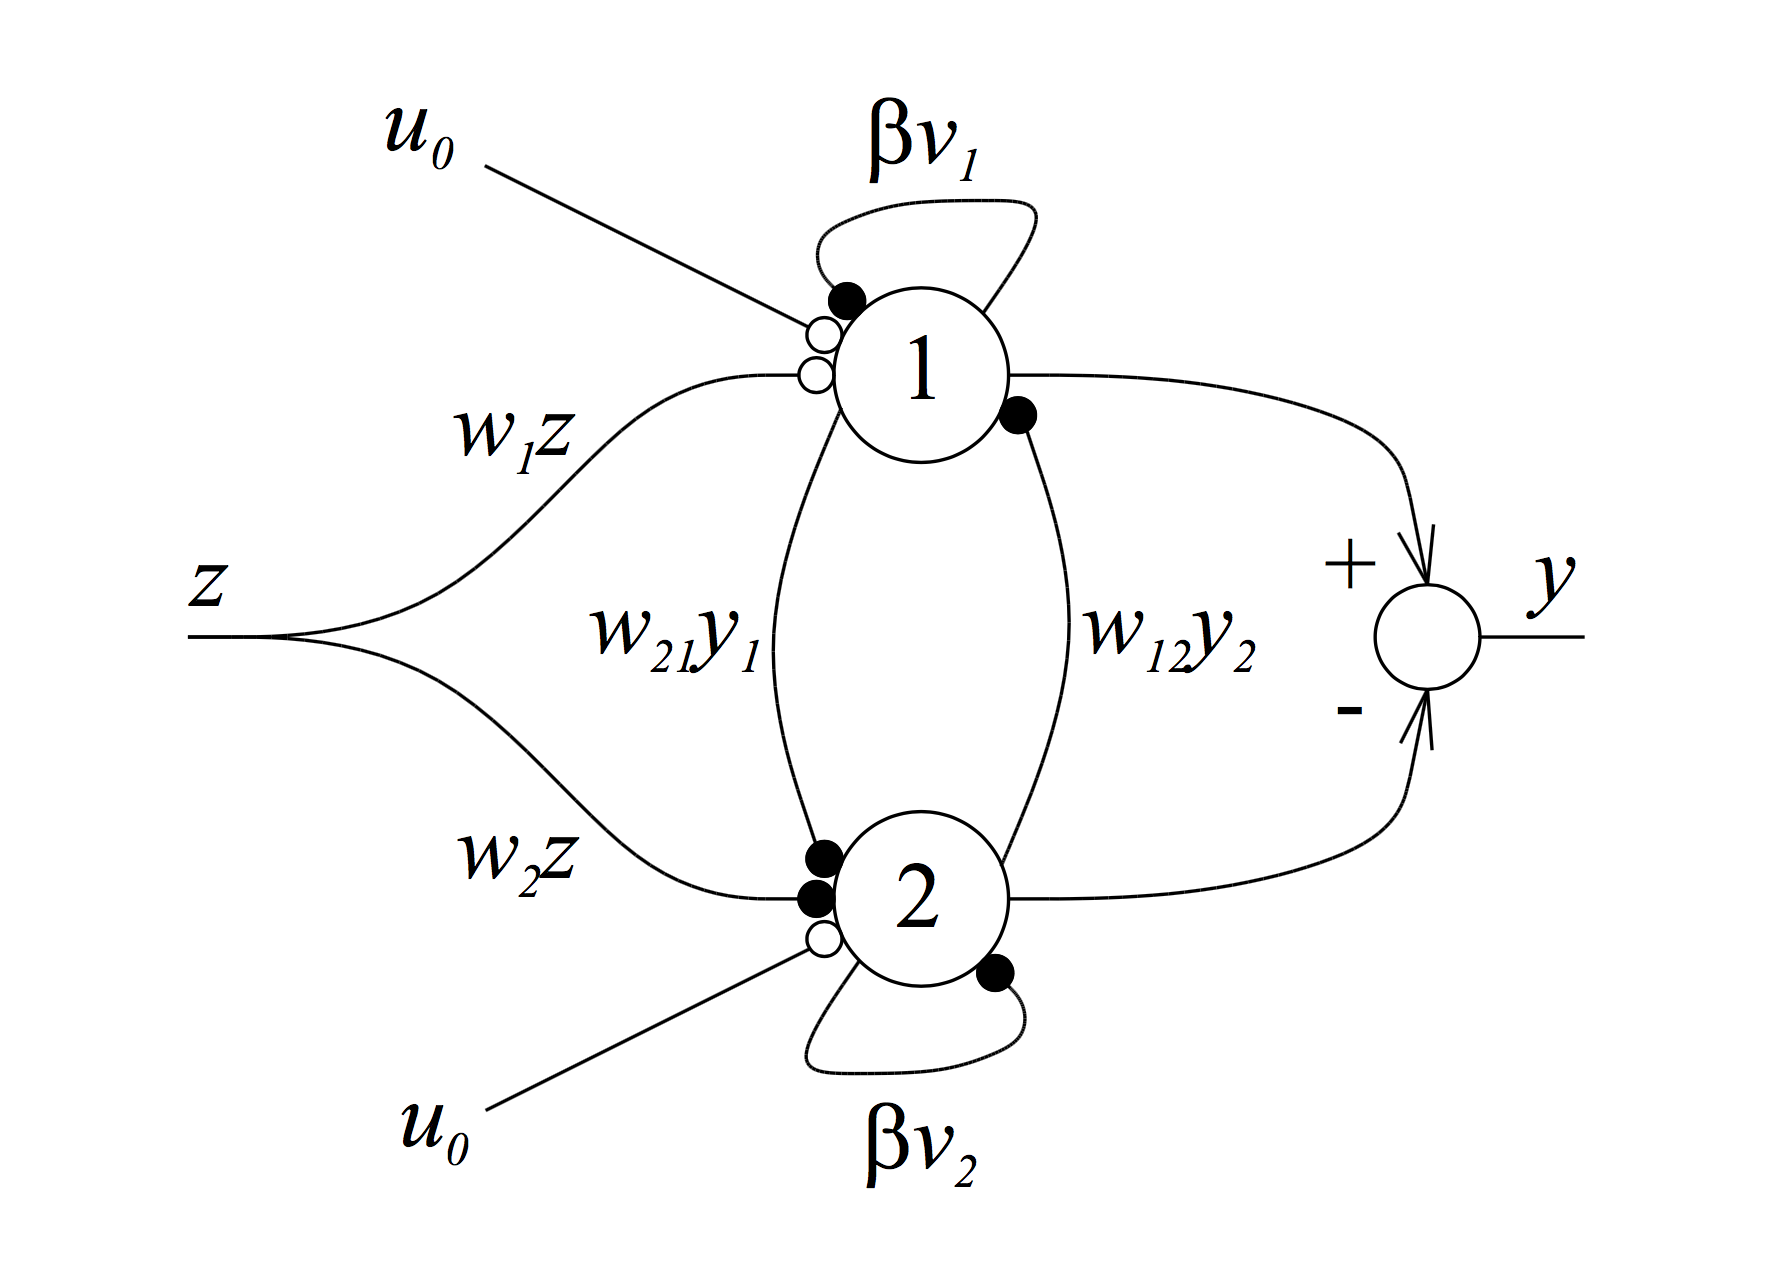
\includegraphics[width=0.75\textwidth]{include/figure/matsuoka.png}
    \caption{The Matsuoka model of a half-centre CPG \cite{CPGwolff}, with parameters explained in Table \ref{tab:parameters}.}
    \label{fig:matsuoka}
\end{figure}

The setup of the Matsuoka model is shown in Figure \ref{fig:matsuoka}, with the parameters as described in Table \ref{tab:parameters}. The behaviour of the model is described by the following equations \cite{CPGequations}:

\begin{align}
    \tau_u \dot{u}_i &= -u_i - \beta v_i + \sum^{n}_{j=1} w_{ij}y_j + u_0, \\
    \tau_v \dot{v_i} &= -v_i + y_i, \\
    y_i &= \text{max}(0, u_i), \\
    o &= y_2 - y_1
\end{align}

where the model is simulated by integrating over time using Euler integration and timestep $\Delta t$ and $\dot{u}_i$, $\dot{v}_i$ from above in:

\begin{align}
    u_i(t + \Delta t) &= u_i(t) + \Delta t \dot{u}_i, \\
    v_i(t + \Delta t) &= v_i(t) + \Delta t \dot{v}_i.
\end{align}

\begin{table}[htbp]
    \centering
    \begin{tabular}{|c|p{6.5cm}|c|c|}
         \hline
\textbf{Parameter} & \textbf{Description} & \textbf{Initial value} & \textbf{Comment} \\ \hline
$z_i$ & input of neuron i &  & oscillating  \\ \hline
$u_0$ & external tonic input & 1.0 &  \\ \hline
$u_1$ & inner state of neuron 1 & 0.0 & fixed \\ \hline
$u_2$ & inner state of neuron 2 & 1.0 & fixed \\ \hline
$v_1$ & auxiliary variable measuring the degree of self-inhibition of neuron 1 & 1.0 & fixed \\ \hline
$v_2$ & auxiliary variable measuring the degree of self-inhibition of neuron 2 & 0.0 & fixed \\ \hline
$\beta$ & modulation parameter & 2.5 &  \\ \hline
$w_{ij}$ & weights connecting neuron j to neuron i & -2.0 &  \\ \hline
$y_i$ & the output of neuron i & 0 & \\ \hline
$\tau_u$ & time constant & 0.025 &  \\ \hline
$\tau_v$ & time constant & 0.3 &  \\ \hline
$o$ & the output of the oscillator & & \\ \hline
    \end{tabular}
    \caption{The parameters used in the Matsuoka model of a half-centre CPG.}
    \label{tab:parameters}
\end{table}


\subsubsection{Model of CPG Network} \label{CPGnetwork}
%Combining different CPG neurons on a network to model a human where each Neuron is a DoF.

Coupling multiple CPGs into a network makes it possible to model more complex structures, such as an animal or a human. This can be done by connecting the output of one neuron to the input of another. This project investigatex the walking behaviour of a human implemented on a humanoid robot, thus human behaviour can be modelled by looking at the movement in different joints of the body, corresponding to the joints of the humanoid robot. Since the output of a CPG is one-dimensional over time, and human movement is three dimensional, one can imagine modelling the movement in each dimension with a separate CPG. The output signals can then be superimposed to obtain the total movement.


\subsubsection{Choice of Input to Oscillator} \label{choiseOfInputToOscillator}
%The different models (summing output and weights). Asyncronous vs syncronous.
%2.1.3 in old report
Each of the neurons in a CPG network have inputs ($z_i$) that are affected by the output of the other neurons ($o$). One can imagine that all neurons are fully connected, but by setting the weight between two neurons to zero, that weight is \textit{removed}. The input to the neurons can be calculated in different ways, one way inspired by Liu et.al. \cite{liu} is to define the inputs to neuron $i$ as
\begin{align}
z_1 &= \sum_{j \text{ neighbour of } i} a_{ij}u_j, \\
z_2 &= 0.
\end{align}
Another implementation inspired by Shan et.al. \cite{shan} defines the inputs as
\begin{align}
z_1 &= \sum_{j \text{ neighbour of } i} a_{ij}[y_j]^+, \\
z_2 &= \sum_{j \text{ neighbour of } i} a_{ij}[y_j]^-,
\end{align}
where 
\begin{align}
[y_j]^+ &:= \text{max}(y_j,0), \\
[y_j]^- &:= \text{min}(y_j,0).
\end{align}

Neurons can also be affected by an external tonic input ($u_0$). The amplitude of the oscillation in the CPG is proportional to the tonic input. If the input is oscillatory, the oscillator will lock to the frequency of the input. When the input is removed, the oscillator will smoothly return to the original frequency \cite{CPGwolff}.


\subsection{Optimisation Using Genetic Algorithm}
A CPG alone might not achieve satisfactory results, as the parameters in the CPG or network might need to be tweaked and optimised to achieve the desired behaviour. A commonly used technique for optimising behaviour is to use reinforcement learning to improve the model based on an external measure of success. This project uses a Genetic algorithm (GA) as a reinforcement learning technique to achieve desired walking behaviour. A genetic algorithm is an evoutionary algorithm that takes inspration from natural selection implemented as an optimisation problem \cite{GAHauert}. 


\subsubsection{Genome}
%Difference between using only weights or the entire CPG network as genome.


The \textit{genome} is a set of parameters that defines a proposed solution to the problem that the GA is trying to solve. One can imagine various different genomes when optimising the behaviour of a CPG, for instance the internal parameters in the CPG, shown in Table \ref{tab:parameters}. The connection weights between neurons in a CPG network, as described in Section \ref{CPGnetwork}, could also be used to account relation between CPGs in a network.

\subsubsection{Operators}
%Init population, simulate behaviour, evaluation, selection, mutation, permutation
The basic implementation of a GA is in summary; initialise the population, simulate the behaviour, evaluate success, selecion process, mutation and permutations, repeat until converge. A more detailed description can be found in \cite{wahde}. The evaluation process, also known as the \textit{fitness function}, produces a fitness score which is the measurement the success of the individual. Since this project investigates walking behaviour in a humanoid robot, a fitness function may include e.g.; distance walked, time walked, stability, falling, walking style, etc.

% METHODS
\newpage
% CREATED BY DAVID FRISK, 2016
\section{Methods}
This section introduces the methods used throughout this project, along with a description of the tools and setup of the simulations. The approach is to collect data from human movement to use in a pre-evolution. Then use the pre-evolved model when preforming simulations on a Bioloid robot model, and later in the physical robot. Much of the basic simulation enviroment was provided by a previous research project \cite{studentProj}, which was further developed during this project.

%To be able to achive the goal stated in the introduction, the project was devided into sections. First, data was collected from a human during a walking cycle. The collected data were processed to later be used for simulations. The simulations were prepared and then performed. The results from the simulations were then implemented into the bioloid. All of these sections will be described in more detail in this chapter in a chronological order  }

%Skriv intro till kapitlet, typ vår tankegång; samla data, använda data i preprocessing, använda preprocessed modell i simulering, testa simuleringen på robot.

\subsection{Record Physical Model} \label{recordPhysicalModel}

\subsubsection{Data Collection}
%Robot has 18 DoF, divided into 8 joints. Record human data from corresponding joints on human.
%Using mobile phones, easy good accelerometer. LiU sensor fusion, export CSV. Putting phones in socks, taping to joints.

%Recorded walking cycle. Jump before start of each cycle as init signal.

%Gather and assemble hardware needed.
%Setup hardware/software interface to collect data.
%Find ideal amount of sensors and their location.
%Gather movement data.

The Bioloid robot has 18 Degrees of Freedom (DoF), which is divided on 8 different joints. These joints can be seen in Figure \ref{fig:Robot_Joints}. To gather data from a human during a walking cycle, accelerometers were strapped to the human in the joints corresponding to the joints of the Bioloid robot, as seen in Figure \ref{fig:Human_Joints}. Smartphones with the app \textit{Sensor Fusion} \cite{sensorfusion} was used to collect the accelerometer data. Using mobile phones enabled easy access to many high quality sensors, and the app provided an interface to export raw sensor data directly to CSV format. The phones were strapped to the joints shown in Figure \ref{fig:Human_Joints}. A walking cycle was initiated with a jump, to find a clear correlation in initialisation between devices, making it easy to extract and allign the signals. More than one walking cycle was recorded during the same session separated by the initialisation signal.
\begin{figure}[H]
    \centering
    \begin{subfigure}[b]{0.5\textwidth}
        \centering
        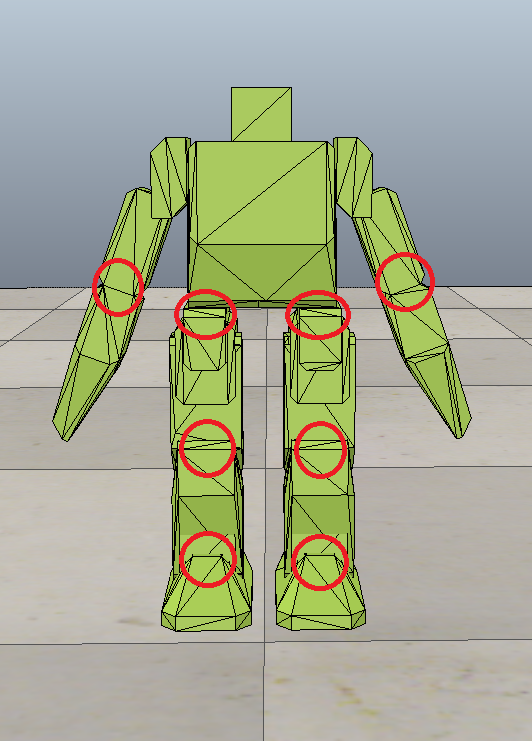
\includegraphics[scale=0.50]{include/figure/Robot_Joints.PNG}
        \caption{Bioloid with joint locations indicated by red circles. }
        \label{fig:Robot_Joints}
    \end{subfigure}%
    ~ 
    \begin{subfigure}[b]{0.5\textwidth}
        \centering
        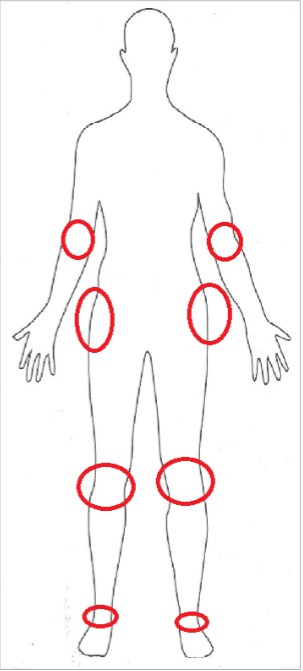
\includegraphics[scale=0.50]{include/figure/Human_Joints.PNG}
        \caption{Human body with accelerometer locations indicated with red circles.}
        \label{fig:Human_Joints}
    \end{subfigure}
    \caption{Joints examined during data collection}
    \label{fig:RLH1}
\end{figure}
\subsubsection{Data Processing}
The recorded data from the walking cycles were processed to align the data between devices and extract walking cycles. All signals were normalised to account for different sensitiveties between sensor models, thus removing bias.


%The X,Y and Z acceleration directions from the joints correkating to the initialization signal were extracted  Once the data was cleared of most noise and the XYZ was extracted, it needed to be normalized because of the fact that the different mobile phones had their differences in the data collected which would lead to bias in the data if not normalized. The results after data collecting and processing was plotted in a graph to give a visual representation, see Figure \ref{fig:AllCyc}   }\\


%Process movement data to be free from noise and possible to use for future steps

%Read recorded data and extract XYZ in joints correlated according to init signals (start at same time). Normalise data to reduce bias from different devices


\subsection{Pre-Evolution}

\subsubsection{Evolve to Fit Physical Model}
%Evolving the mathematical model to fit the physical gathered data 
To leverage the behaviour of humans using the collected data presented in Section \ref{recordPhysicalModel}, a pre-evolution was constructed. The main goal of the pre-evolution was to adopt the output of a CPG network to fit the behaviour of the recorded data. Performing the pre-evolution in an environment not requiring any graphical interface or control of a robot model would hypothetically converge faster then using a full-scale simulation environment. Using an optimised model when performing later simulations on a robot model would then ideally evolve a better behaviour faster.


\subsubsection{Model Construction}
%Model as a CPG using Matsuoka and GA.
The initial intention was to use the same model in the pre-evolution as in the evolution in the robot simulation. But it was discovered that the existing simulation and evolution environment were too highly linked together, meaning that it was easier to construct an independent pre-evolution model. The model was higly inspired by the existing environment, using the Matsuoka model described in \ref{modelOfNeuralOscillator} to model the CPGs and initial parameters as presented in Table \ref{tab:parameters}. The pre-simulation investigated two different types of genomes. In the first case only the connections between the neurons in the CPG network was used, while in the second case all the parameters of the Matsuoka model was used.

The pre-simulation was performed on a CPG network of 18 neurons, corresponding to the 18 DoFs on the humanoid robot. The neurons were initialised fully connected using a connection matrix with random values. The input model by Liu introduced in Section \ref{choiseOfInputToOscillator} was used, the outputs were initiated randomly, since it was required that the output values were initialised to non-zero values to start the evolution. The CPG model was simulated over 20 seconds with a timestep of 0.01 seconds, corresponding to the time of one recorded walking cycle, generating an output signal. The population size was varied between simulations between 20-40 individuals, and full-scale evolutions were made with 500-1000 generations.


\subsubsection{Fitness and Reinforcement}
%Use correlation as fitness functuion. 
When simulated, the CPGs were evaluated by assigning each neuron to a DoF, then comparing the output signal to the corresponding recorded reference signal. This was done by taking the \textit{correlation} between the output signal and the reference signal. A correlation of 1 mean full correlation (identic signals) and a correlation of -1 indicates no correlation (signals shifted half a period). The fitness score was aquired by taking the absolute value of the \textit{lowest} correlation between an output DoF and a reference DoF in an individual, the idea being to maximise the worst correlation in each population. Other fitness functions can be imagined as measuring different similarities between the signals, analysing the moments of the correlation distribution, analysing symmetry between signals, evaluting each DoF individually instead of depending on the rest of the individual, etc. 

Once evaluated, the next generation was chosen by tournament selection, with a tournament size of a fifth of the population size. Elitism was implemented not to loose the best individual, mutations and permutations were randomly applied to the rest of the population. 

\subsection{Implementation of the GA and Simulation}
The method used to evaluate and iterate the weights for the CPG was a standard genetic algorithm, with elitism, tournament selection, mutations and crossovers. The specific parameters of the model can bee seen in Appendix \ref{app:GAparametersPrimary}. The fitness of each individual was evaluated by measuring the distance a simulated 3D model of the Bioloid could travel. The simulated Bioloid accepted input signals in the same way as the physical one. This made it possible to accurately measure and analyse the movement of the robot without having to connect it to the actual Bioloid, thereby speeding up the simulation and the algorithm. However, it came at the cost of disrepancies between the simulated enviroment and the real world. The chosen simulation environment in this project was V-REP \cite{v-rep}, in which a model of a Bioloid robot was imported. Based on how far the simulated Bioloid was able to walk, each individual was assigned a fitness value and compared to the rest of the evaluated individuals. Several fitness functions were evaluated, and the one found to be the most useful was one that multiplied the greatest distance the robot travelled, with the lowest height of the robot. This was to prevent the robot from falling over while still rewarding behaviour that pushed it forward. However, based on the specifics of the simulation, such as stability and DoF, it could be varied for a more specialised approach, such as simply the distance travelled forward.

\subsubsection{Configuration of V-REP}
V-REP efficiently allowed for the import and simulation of the Bioloid robot. The 3D model of the Bioloid was the same as used in the previous project \cite{studentProj}, and can be viewed in the V-REP enviroment in Figure \ref{fig:freeBioloid}. After loading the model into a specific V-REP scene, the GA automatically sent signals into the simulation as soon as it started. The V-REP platform also allowed for an arbitrary number of joints/servos to be simulated, meaning the algorithm could be focused to generate patterns only for a select number of servos.  
\begin{figure}[htbp]
    \centering
    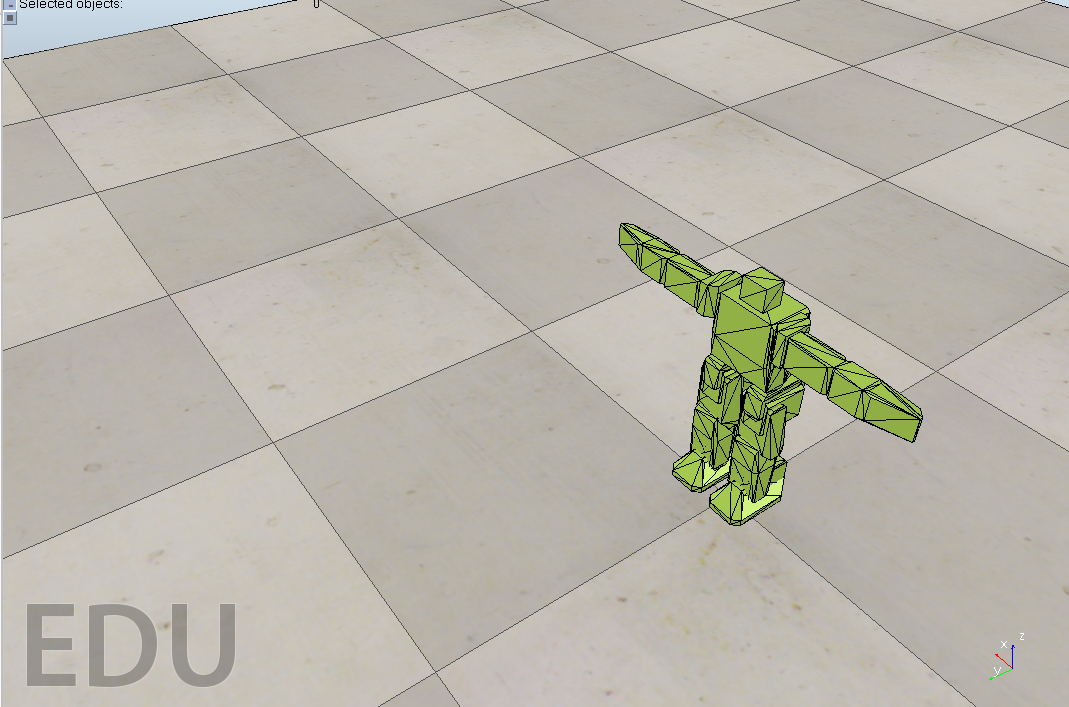
\includegraphics[scale=0.25]{include/figure/freeBioloid.png}
    \caption{The 3D Bioloid model used in the V-REP simulation enviroment.}
    \label{fig:freeBioloid}
\end{figure}
\subsubsection{Physical Implementation and Hardware}
The physical Bioloid robot was pre-assembeled into the standard configuration A \cite{bioloidMan}, offering the highest degree of freedom and replication of the human body. The standard control board on the Bioloid was ignored in favor of connecting directly to the servos and controlling them through an application on the computer. This was accomplished by daisy-chaining all the servos together and connecting them to both a power source and a \textit{USB2Dynamixel} \cite{dongle} dongle, which allows for direct computer-to-servo communication. As before, much of the software infrastructure regarding communication was taken from the previous student project \cite{studentProj}, along with some specific software to communicate with the USB2Dynamixel dongle. As the simulated Bioloid in V-REP had higher friction against its surroundings, the physical Bioloid was modified in order to increase friction of its feet against the floor. This was accomplished with simple modelling clay attached to the soles of its feet.
\subsubsection{Simulation Process}

As previously mentioned, the number of simulated servos could easily be changed in the simulation. Two main approaches were used - one where all 18 joints of the Bioloid were simulated, and one where only 8 were considered. Based on the initial hypothesis, a robot with 18 DoF would be better able to replicate human movement and should thus be able to generate the best results. However, the increased degrees of freedom also led to an increased tendency for the robot to topple and fall. Initially, the simulation with all 18 joints simply let the robot orient itself without any external support and attempt to develop a walking gait from there. It quickly became appearent that the full 18 DoF case would be very slow to develop a walking gait, if it did so at all. In order to speed up the process support rods attached to the robot was used, first four, and then two, in order to prevent the robot from falling down but without interfering too much in the evaluation of the fitness. The 4-rod model can be viewed in Figures \ref{fig:4rods}, and the 2-rod model can be see in Appendix \ref{app:model}, Figure \ref{fig:2rods}. The purpose of these was to take the best result from the simulation with four support rods, and insert that into the simulation with two support rods, and then finally insert the best result from there into a simulation with no support, in order to finally reach a stable gait. 

In the case of only 8 joints, the robot was constricted to only move in the forward direction by means of a support arm, seen in Figure \ref{fig:supportArm}. The arm was used to prevent the robot from falling to either side. The purpose of this was to increase its stability and speed up the simulation, sacrificing freedom of movement and possibly a more human-like gait in order to get stable results faster. Of course, the physical robot would then need to be attached to a support beam as well in this case. Based on preliminary results, the robot was also simulated with all 18 DoF and a support arm, to see if it gave any performance improvements in comparison to the 8 DoF case. Each simulation ran for around 50-70 generations with around 30 individuals in each population. The reasons for these parameters were somewhat arbitrary, as they seemed to give a good enough mix of convergence speed coupled with a reasonable runtime (around 5-7 hours).
\begin{figure}
\centering
\begin{subfigure}{0.5\textwidth}
    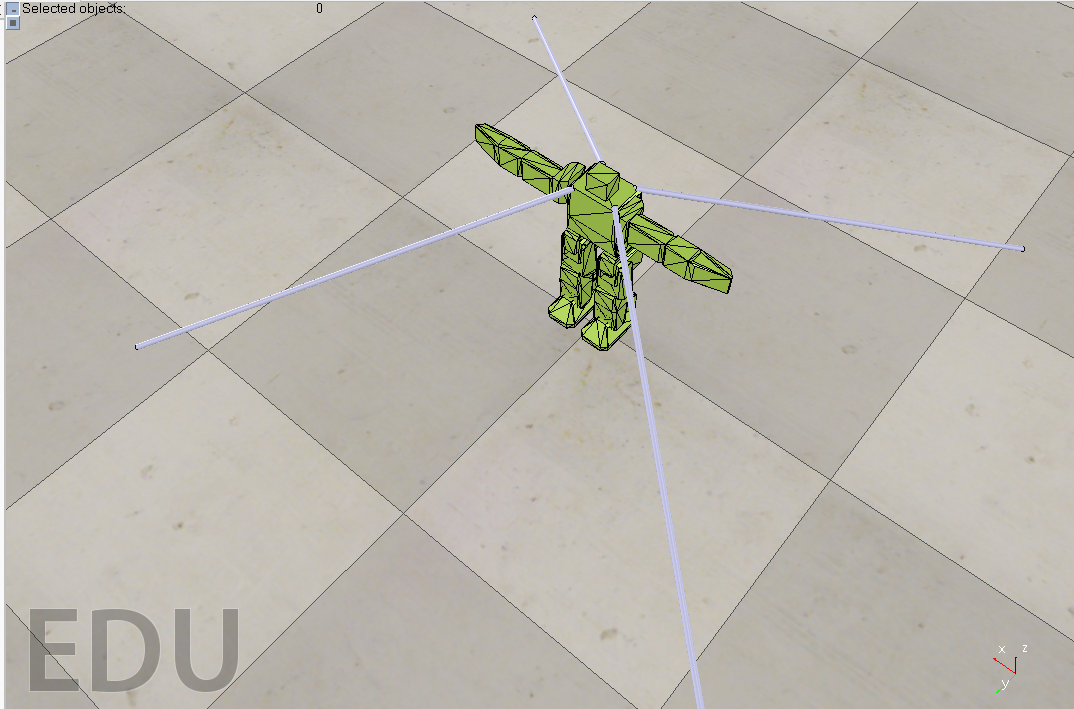
\includegraphics[scale=0.20]{include/figure/4rods.png}
    \caption{The Bioloid model with 4 support arms in the V-REP simulation enviroment.}
    \label{fig:4rods}
    \end{subfigure}
    \begin{subfigure}{0.5\textwidth}
    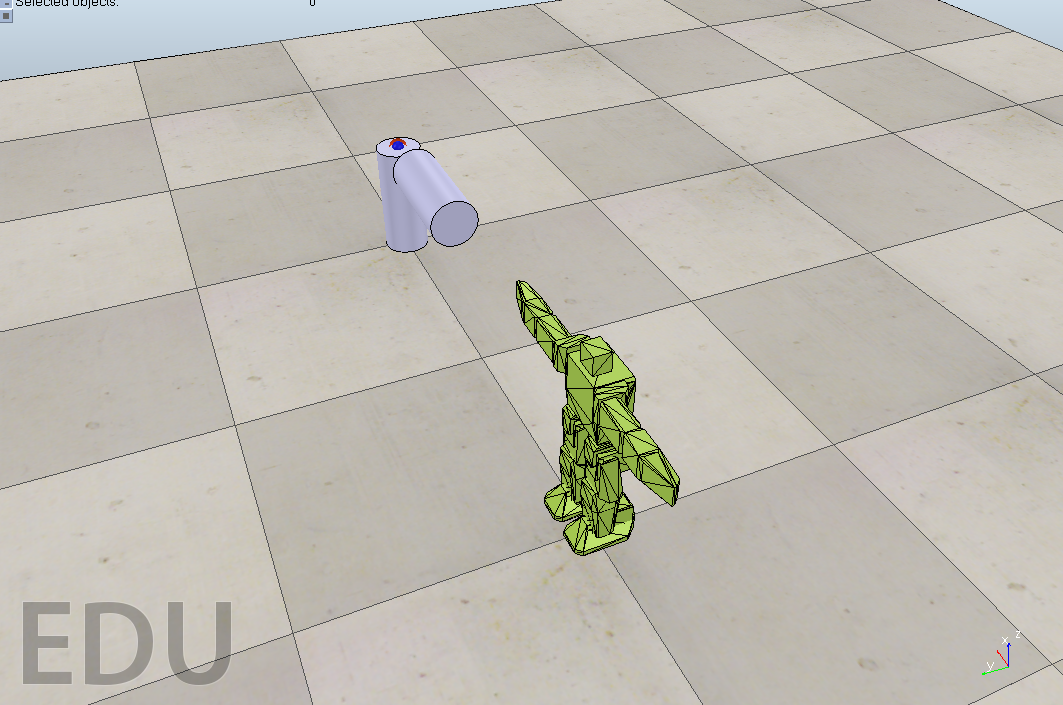
\includegraphics[scale=0.20]{include/figure/supportArm.png}
    \caption{The Bioloid model with the external support arm in the V-REP simulation enviroment.}
    \label{fig:supportArm}
    \end{subfigure}
    \caption{Overview of the different support structures used in the simulation.}
\end{figure}

% RESULTS
\newpage
% CREATED BY DAVID FRISK, 2016
\section{Results}
The results from both the pre-evolution process and the main simulation are presented in this Section. When possible, figures have been used to more clearly represent the data. In the case of the movement of the robot, care has been taken to describe the dynamics as accurately as possible.

\subsection{Processed data}
The processed data was plotted in a graph to identify walking cycles, see Appendix \ref{ProcessedData}. As this plot contained too much information to give a clear image and for clarity, two plots were made containing only the information from the left and right hip's acceleration in the z-axis which was enough to check for a pattern. These plots can be viewed in Figure \ref{fig:WalkingCycles}, where walking cycles can be clearly identified.


\begin{figure}[H]
    \centering
    \begin{subfigure}[b]{0.5\textwidth}
        \centering
        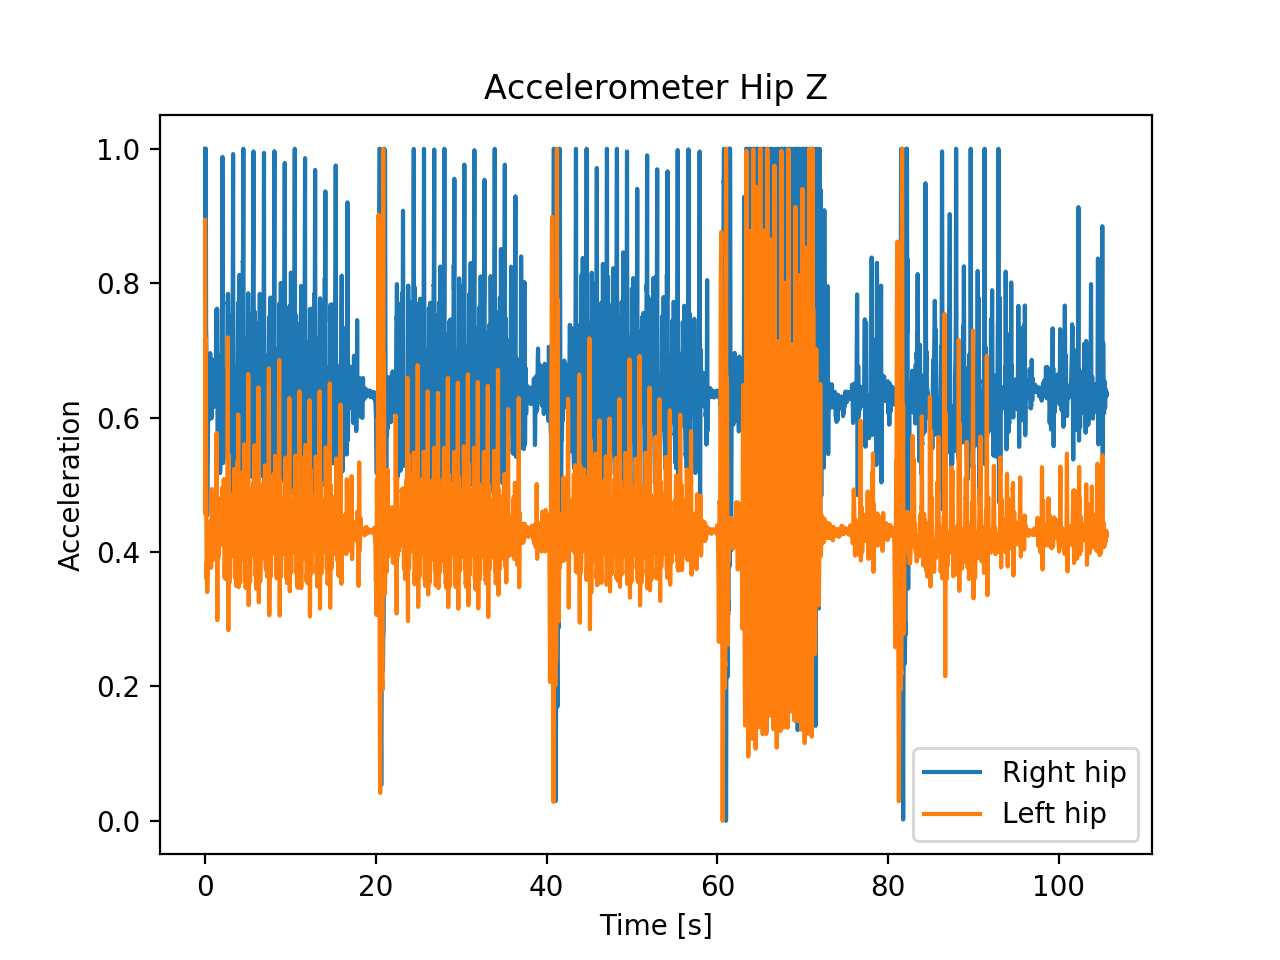
\includegraphics[width=1\textwidth]{include/figure/RLH5.png}
        \caption{Plot of the gathered data from five walking cycles.}
        \label{fig:RLH5}
    \end{subfigure}%
    ~ 
    \begin{subfigure}[b]{0.5\textwidth}
        \centering
        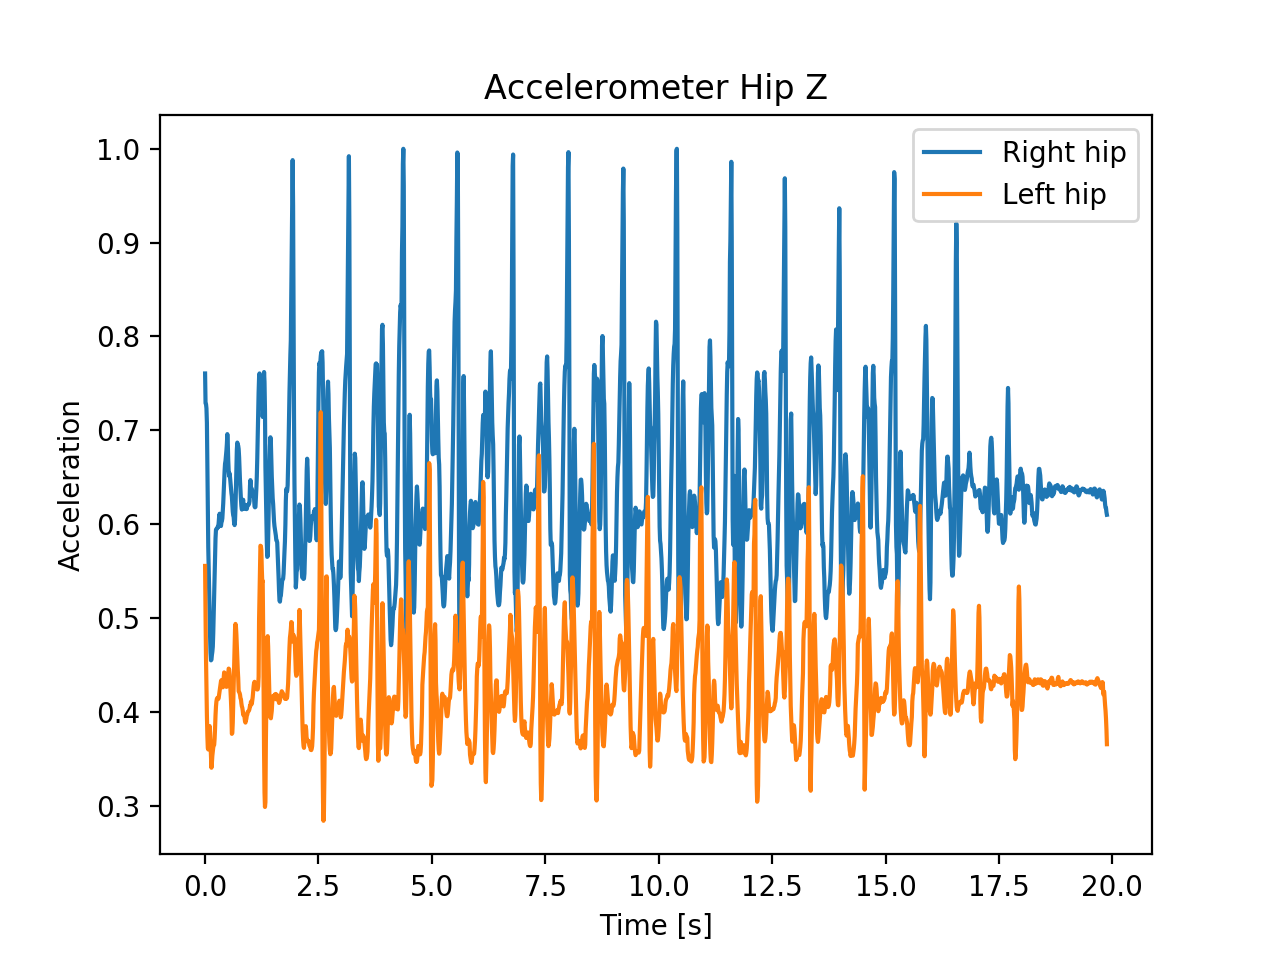
\includegraphics[width=1\textwidth]{include/figure/RLH1.png}
        \caption{Plot of the gathered data from one walking cycle.}
        \label{fig:RLH1}
    \end{subfigure}
    \caption{Processed Data from the recorded walking cycles.}
    \label{fig:WalkingCycles}
\end{figure}

\subsection{Pre-Evolution}
Simulation of the CPG model was done over 20 seconds with a timestep of 0.01 seconds, corresponding to the time of one recorded walking cycle. The population size varied between 20-40 individuals depending on simulations. Full-scale evolutions were made with 500-1000 generations.

\begin{figure*}[htbp]
    \centering
        
    \begin{subfigure}[b]{0.45\textwidth}
        \centering
        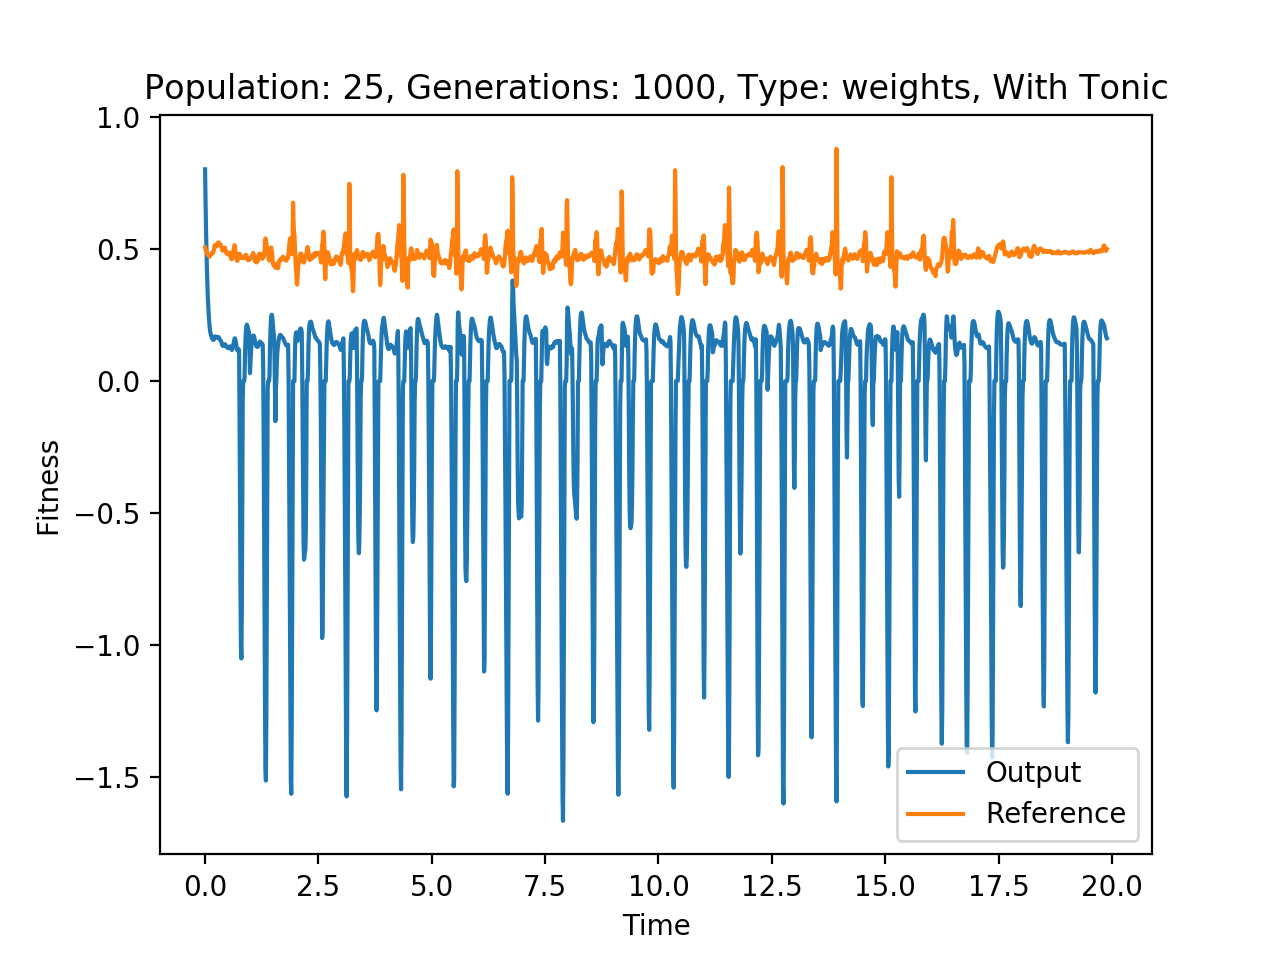
\includegraphics[width=0.95\textwidth]{include/figure/output_pop25_gen1000_type0_with.png}
        \caption{Original version.}
        \label{fig:result_1a}
    \end{subfigure}
    ~ 
    \begin{subfigure}[b]{0.45\textwidth}
        \centering
        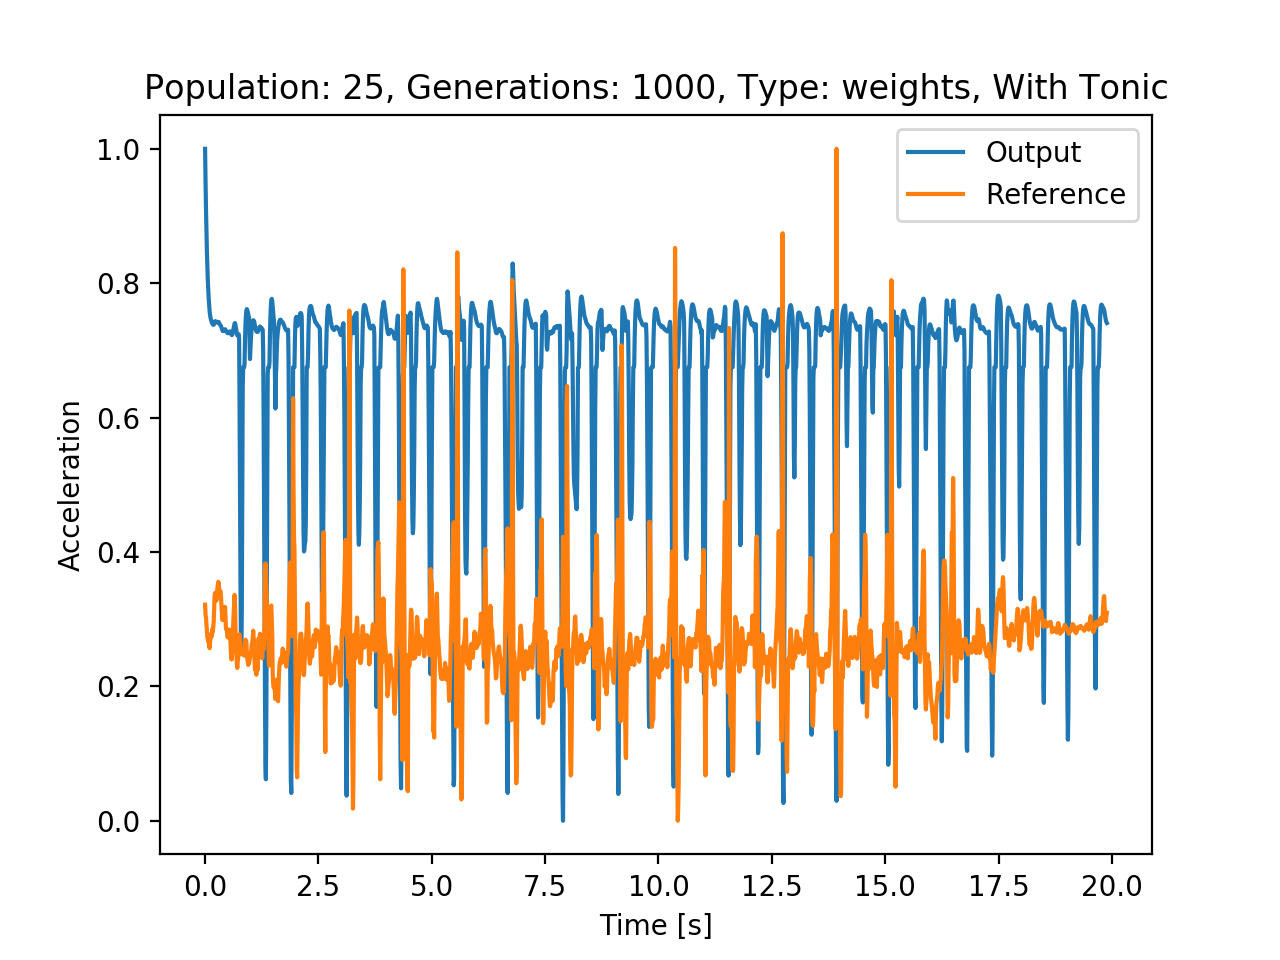
\includegraphics[width=0.95\textwidth]{include/figure/best_individual_output_pop25_gen1000_type0_with_normalised.png}
        \caption{Normalised version.}
        \label{fig:result_1b}
    \end{subfigure}%
    \caption{Output signals of the CPG network.}
    \label{fig:result_1}
\end{figure*}

As seen in Figure \ref{fig:result_1a}, the amplitude of the output signal does not match the amplitude of the reference signal. To easier compare the signals, the output signals were normalised, which can be seen in Figure \ref{fig:result_1b}. It can be seen that the pre-evolution simulation manage to create rhytmic output patterns, but does not manage to match the amplitude of the reference signals significantly. This is confirmed by the fitness scores, shown in Figure \ref{fig:fitness_1}. The fitness is maximally around 4\% correlation, which is quite low, since they ideally should be fully correlated. When using the entire Bioloid as type, it refers to using both the internal parameters in the CPG as well as the weights between them as genome. Further results are shown in Appendix \ref{resultsOfPreEvolution}.

\begin{figure*}[htbp]
    \centering
    \begin{subfigure}[b]{0.5\textwidth}
        \centering
        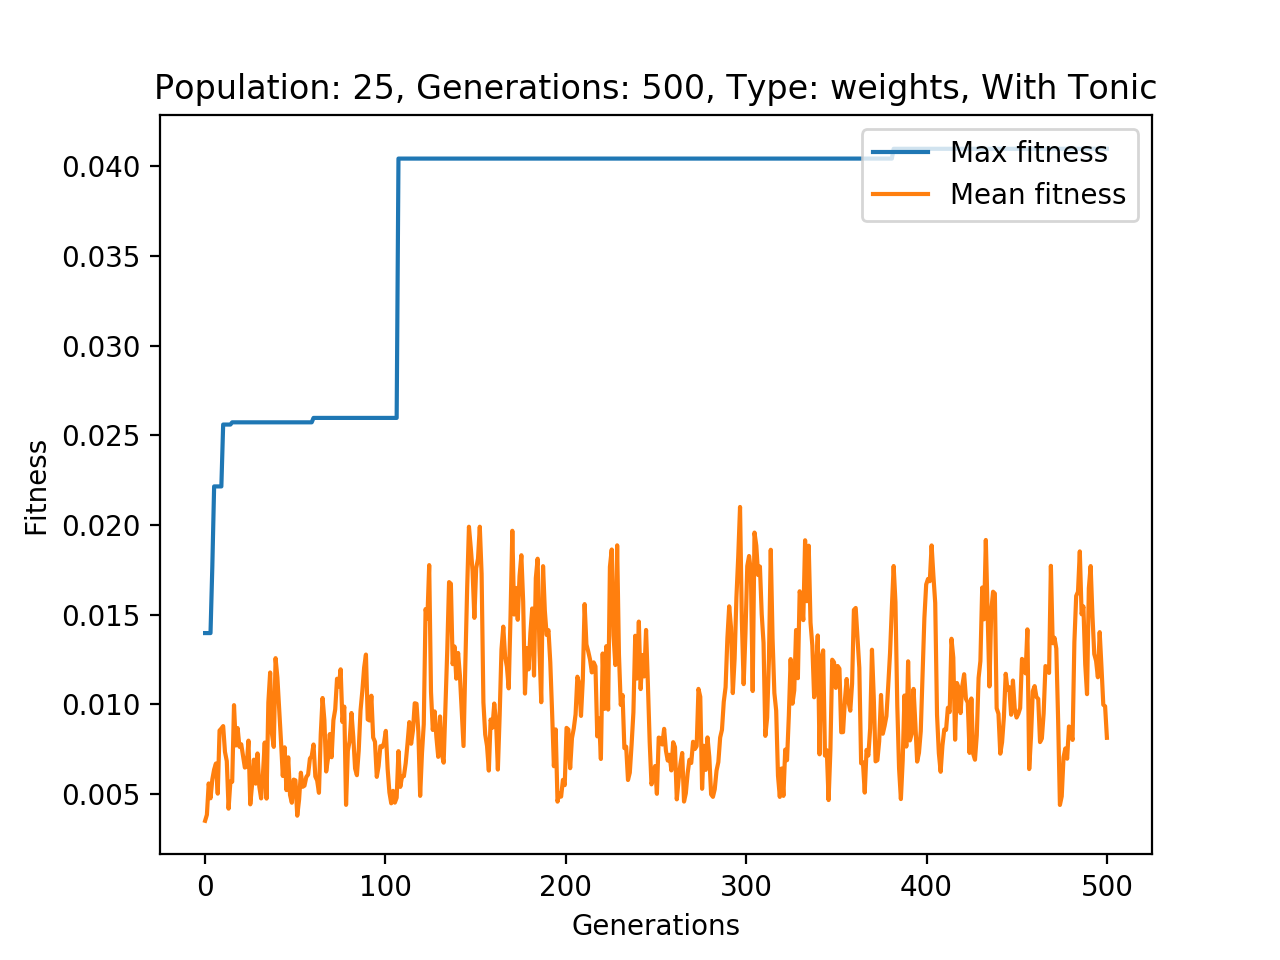
\includegraphics[width=1\textwidth]{include/figure/fitness_over_time_pop25_gen500_type0_with.png}
        \caption{Only weights. \vspace{0.5cm}}
        \label{fig:fitness_1a}
    \end{subfigure}%
    ~ 
    \begin{subfigure}[b]{0.5\textwidth}
        \centering
        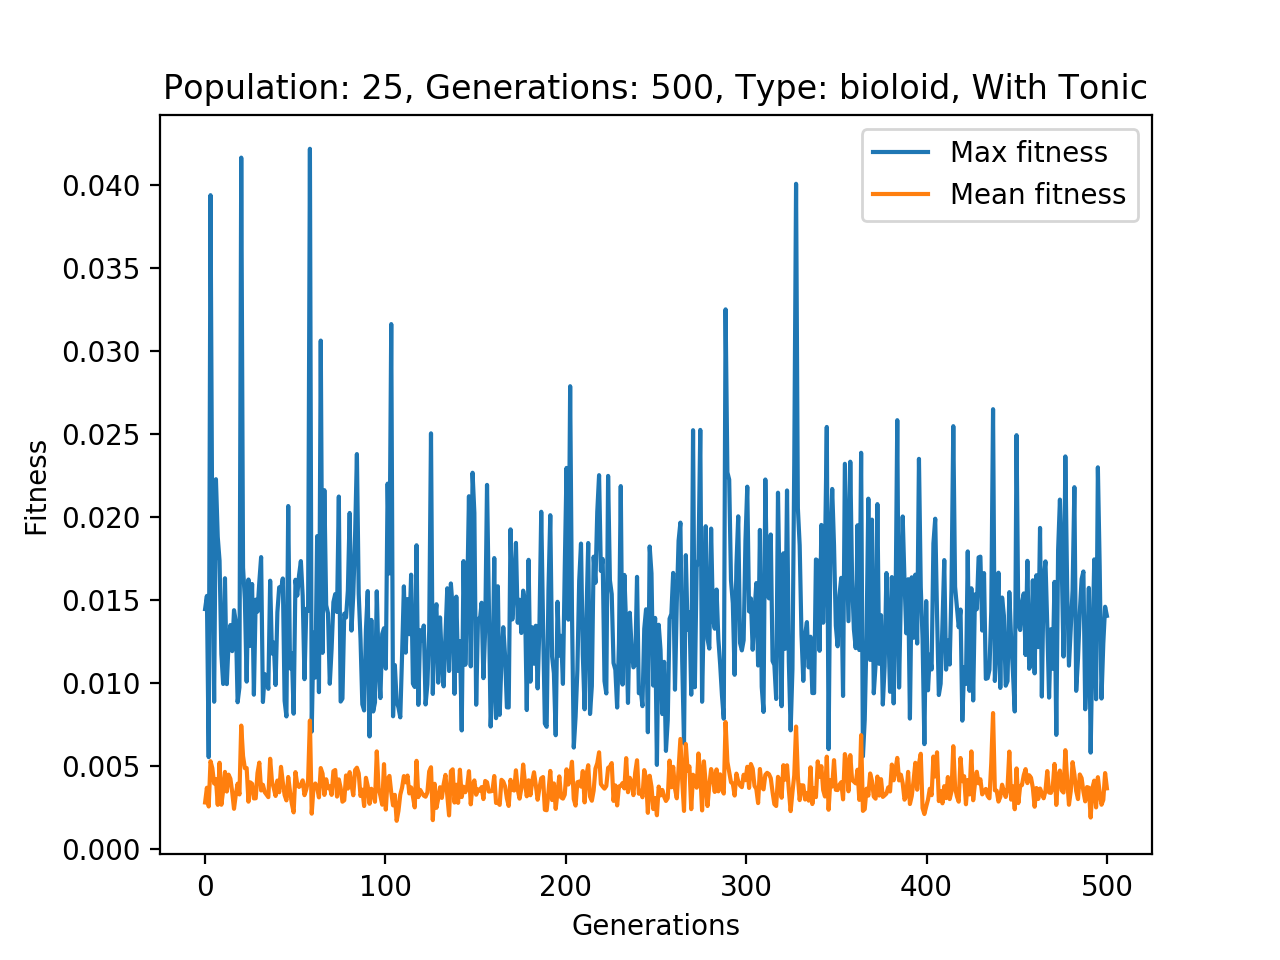
\includegraphics[width=1\textwidth]{include/figure/fitness_over_time_pop25_gen500_type1_with.png}
        \caption{Entire bioloid, both weights and internal parameters.}
        \label{fig:fitness_1b}
    \end{subfigure}
    \caption{The evolution of the fitness function.}
    \label{fig:fitness_1}
\end{figure*}


\subsection{Simulation}
In the case of the 18 DoF simulation with the support rods attached to the Bioloid robot, the Bioloid never achieved a walking cycle. From the start, the simulation with four rods did not properly converge into a stable cycle, which propagated to the case with two support rods, and further in the simulation with no support rods. The initial values were evidently too unstable for the robot to support itself, even if it did display some rudimentary capability to throw itself forward rather than backward. With these results, efforts were focused on the simulations where the external support arm was present, both with 8 and 18 degrees of freedom. Here the results are more closely overlapping, but as expected the 18 DoF simulation is more unstable than the 8 DoF simulation. 

Neither simulation achieves a walking cycle comparable to the data gathered from the accelerometers, which means it is quite far off from a humanoid walking cycle. Both movement cycles seem to mainly exploit the fact that in the simulation, it is possible to inch the robot forward by extending one leg and wobbling the foot servo, generating a small amount of friction that slowly pulls the robot forward. However, this does not hold up when applied to the physical Bioloid, since the friction coefficient is completely different, caused by the reality gap. This can probably be tweaked by changing the friction material (modeling clay in this case) to something with less grip, possibly allowing the Bioloid to inch forward like in the simulation.

%DISCUSSSION
\newpage
\section{Discussion}
\label{discussionSec}

When using the entire bioloid as a type during the pre-evolution generated a somewhat unexpected behaviour in the fitness function, as seen in Figure \ref{fig:fitness_1a}. Since the implementation is using elitism, we would expect the maximum fitness to be non-decreasing. The fitness is measured at the end of a simulated generation, and the correlation is an aggregate of the similarity between the output signal and the reference signal over time. Hence, when using the internal parameters as genome, their performance depend on the earlier input values to the CPG, which are constantly changing between generations as the model is updated. An elite individual can therefore never be guaranteed to be the best individual both in current and in future generations. Compared to using only the weights as genome, where the internal parameters in the GPGs are reset between each simulation run, the individuals always have the same starting conditions for each generation, and the elite individual can be maintained.

Why are these results not better then? To start with, the simulations were only made over maximum 1000 generations with a population size of 30. Even if the fitness function seem to converge already between 100-200 generations, a more conclusive result could be achieved by simulating the model over longer time with higher population size. Also, since the output signal does not adapt to the amplitude of the input signal, one might reason that it could be some problems in the implementation of the CPG or GA models. Building a CPG model with a GA from scratch took a great amount of time. Much of the time was spent to understand the specifics of the models and algorithms and getting a working prototype, and less time was spent optimising the model. With more time, further investigations of the functionality and optimality of the model could be made. Furthermore, it would probably be more reasonable to optimise each DoF independently instead of all DoF collectively in an individual.

If we now look at the walking cycle GA, while the robot does manage to move forward, it is far from the walking cycle captured from the accelerometers. A simple solution might be to just increase the simulation time - after all, given infinite time, surely the simulation would generate a walking cycle? While this is true, there are several other factors that explain the discrepancy by the desired output and the achieved output. The first aspect is the differences between the simulated robot and the physical one. As mentioned before, the friction is a major difference, but also the movement and dynamics of the robot, creating a major reality gap. In real life, the servos of the Bioloid are heavy, quite stiff and unable to move particularly fast. The 3D model, by comparision, is lightweight, with joints that swivel and move far faster than the real robot ever could. Not only does this result in a 3D simulation that is more unstable  (in terms of standing without falling, etc.), but also that the results gained from it is troublesome to translate in the real robot. In the current state, the simulation tends to exploit small, single-joint movements to propel itself forward. But looking at the overall scope of the project, we desire movements that can efficiently transfer the accelerometer data to the simulation, and finally to the real robot. That implies that we need movement cycles robust enough to translate between all three levels, and it is resonable to assume that would be dynamics that utilize quite large movements of several joints together - like moving all the joints in one leg at once. In order to counteract this, it would be well worth the time to fine-tune the Bioloid model and the V-REP enviroment, and making sure the simulation enviroment aligns as closely to the real world as possible. However, not all efforts should be focused on the 3D enviroment either. More care needs to be taken in regards to the GA parameters, and the fitness function used. In the current GA, the fitness function does not sufficiently punish inefficient walking modes, such as favoring one leg over the other, not keeping the torso straight, or moving the arms in a way that counteracts the forward motion. Finally, a deeper  understanding of both GA:s and CPG networks would be required to utilize the full potential of the methods. It is likely that a better choice of parameters in both the GA and CPG would have yielded better results, since they were chosen quite arbitraily in the current implementation. The pre-processing for the CPG weights took a lot of development and simulation time, and in the end the results did not compare to the time spent developing it. It was also not until the later stages of the project that the oscillating input to the Matusoka was considered, where an earlier implementation could have lead to better results and perhaps allowed us to skip the pre-processing of the CPG altogether. It is also possible that a GA does not result in the best performance, and instead some other form of reinforced algorithm should be considered. However, despite all this the simulation showed clear signs of improvement during the runtime. Due to deadlines the simulation runtime was limited, but it would be interesting to see what results a week-long simulation would generate. A common behaviour of GA:s is to be stuck in a behaviour for a considerable amount of time, and then stumble upon a behaviour with considerably higher fitness. Such jumps were not observed in our simulations, reinforcing the idea that the GA needed more fine-tuning, but perhaps also more runtime.

% CONCLUSION
\newpage
% CREATED BY DAVID FRISK, 2016
\section{Conclusion}
In the end, the simulations did not generate the desired movement patterns, even if they moved the robot forward. Despite this, it is the opinion of the authors that the chosen methods are valid and can potentially result in faster and more ''natural'' walking cycles than what a randomly seeded simulation would. However, greater care needs to be taken when considering the simulation environment, runtime, parameters for both the CPG and the GA, and the fitness function. The authors encourage anyone interested to continue building on this project, as it is a great learning experience regardless of the generated results. The code base and this report should serve as a sufficient base for anyone considering to continue this work.

%FURTHER WORK
\newpage
\section{Further Work}
In order to most efficiently improve on the project, CPG model and the fitness function should be the main priority. For instance, incorporating a oscillating tonic input in the CPG model, and a greater focus on punishing unwanted behaviour via the fitness function. The V-REP model should be modified to more accurately reflect the Bioloid robot, as should the interaction between the Bioloid model and the simulation floor. Beyond this, increasing the modularity of the codebase would greatly improve the flexibilty of the project and allow for greater changes to the base of the project. In its current iteration, the GA, V-REP, parameters such as number of used servos, the fitness function, and function used to replay and evaluate generated individuals are all heavily intertwined and in some cases hardcoded. As a result, it is not possible to evaluate other reinforcement algorithms, other simulation enviroments, etc. Evaluation and fine-tuning of the GA and CPG parameters would also be of great importance, as would a more accurate simulation envionment.

% REFERENCES / BIBLIOGRAPHY
\cleardoublepage
%\addcontentsline{toc}{Section}{Bibliography}
% CREATED BY DAVID FRISK, 2016
\begin{thebibliography}{69}
\bibitem{CPGHauert}
Sabine Hauert. \textit{Bio-mimetic
Robot Control}, Lectures in Bio-Inspired Artificial Intelligence at University of Bristol, February 16, 2016

\bibitem{GAHauert}
Sabine Hauert. \textit{Artificial Evolution}, Lectures in Bio-Inspired Artificial Intelligence at University of Bristol, February 9, 2016

\bibitem{CPGmodels}
G. M. Shephard. \textit{Neurobiology, 3rd ed. 1994, ch. 20, pp. 435–451.}

\bibitem{matsuoka}
K. Matsuoka. \textit{Mechanisms of frequency and pattern control in the neural rhythm generators}. Biol Cybern, vol. 47, no. 2–3, pp. 345– 353, 1987.

\bibitem{CPGequations}
G. Taga, Y. Yamaguchi, and H. Shimizu. \textit{Self-organized control of bipedal locomotion by neural oscillators in unpredictable environ- ment}, Biological Cybernetics, vol. 65, pp. 147–159, 1991.

\bibitem{wahde}
Mattias Wahde. \textit{Biologically Inspired Optimization Methods: An Introduction}. WIT Press, 2008.

\bibitem{liu}
Guang Lei Liu, Maki K. Habib, Keigo Watnabe, and Kiyotaka Izumi. \textit{Central pattern generators based on matsuoka oscillators for the locomotion of biped robots}. Artif Life Robotics, 12:264–269, 2008.

\bibitem{shan}
Jiang Shan, Cheng Junshi, and Chen Jiapin. \textit{Design of central pattern generator for humanoid robot walking based on multi-objective ga}. In Proceedings of the 2000 IEEE/RSJ International Conference on Intelligent Robots and Systems, volume 3, pages 1930–1935. IEEE.

\bibitem{CPGwolff}
Krister Wolff, Jimmy Pettersson, Almir Heralic, and Mattias Wahde. \textit{Structural Evolution of Central Pattern Generators for Bipedal Walking in 3D Simulation}, October 11, 2006

\bibitem{bioloidMan}
Robotis Inc. \textit{Bioloid Premium Kit Assembly Manual}, \url{http://www.robotis.com/download/doc/BIO_PRM_Humanoid_ASM.pdf}, Accessed 30/10/2017

\bibitem{studentProj}
Helga Kristín Ólafsdóttir et al. \textit{Evolving a human-like gait}, \url{https://drive.google.com/file/d/0By4BzP3-lonJTnJTdmdGSVpJVDg/view}, Accessed 30/10/2017

\bibitem{bioloid}
Trossen Robotics. \textit{Bioloid Premium Robot Kit}, \url{http://www.trossenrobotics.com/p/bioloid-premium-robot-kit.aspx}, Accessed 30/10/2017

\bibitem{sensorfusion}
Fredrik Gustafsson. \textit{Sensor fusion}, Linköping University, \url{https://play.google.com/store/apps/details?id=com.hiq.sensor&hl=en}, Accessed 31/10/2017
\bibitem{v-rep}
Coppelia Robotics, \textit{V-REP Virtual Robot Experimentation Platform}, \url{http://www.coppeliarobotics.com/}, Accessed 31/10/2017
\bibitem{dongle}
Trossen Robotics. \textit{Robotis USB2Dynamixel Adapter}, \url{http://www.trossenrobotics.com/robotis-bioloid-usb2dynamixel.aspx}, Accessed 31/10/2017
\end{thebibliography}


% APPENDICES
%\cleardoublepage
\appendix
%\setcounter{page}{1}
%\pagenumbering{Roman}			% Capitalized roman numbering starting from I (one)
% CREATED BY DAVID FRISK, 2016
\section{V-REP Models}
\label{app:model}
\begin{figure}[htbp]
    \centering
    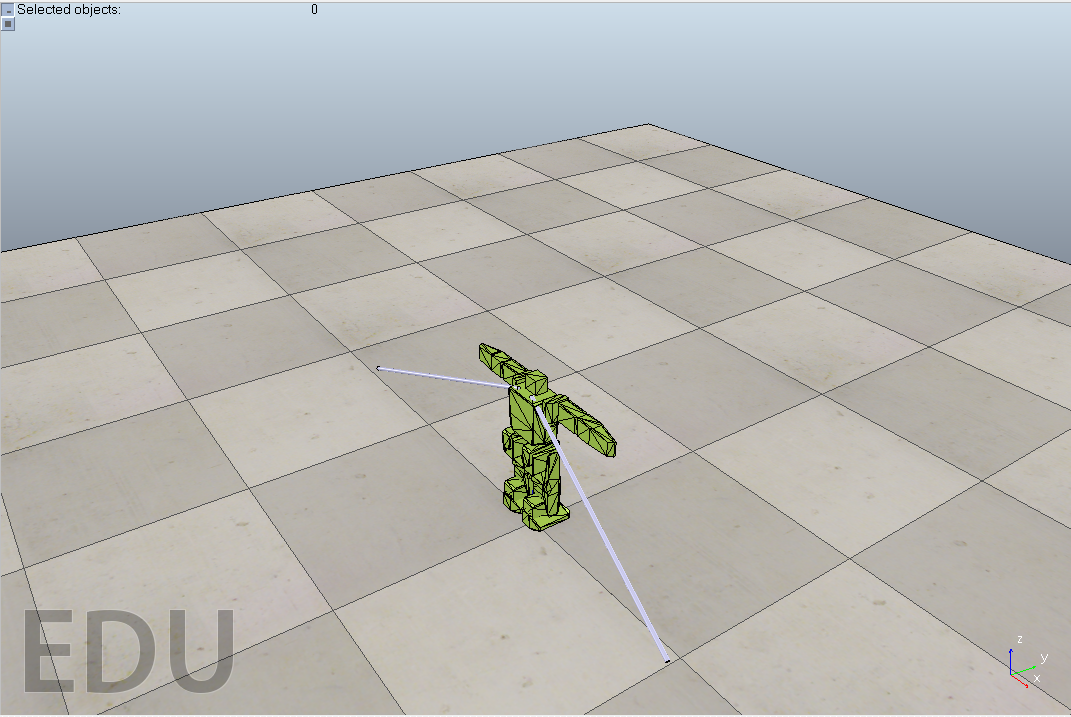
\includegraphics[width=0.35\textwidth]{include/figure/2rods.png}
    \caption{The Bioloid model with 2 support arms in the V-REP simulation enviroment.}
    \label{fig:2rods}
\end{figure}
\section{Parameters for Walking Cycle GA}
\label{app:GAparametersPrimary}
\begin{tabular}{|c|c|}
\hline
nIndividuals & 10 to 30\\
\hline
nGenerations & 50 to 70\\
\hline
pTournament & 0.75\\
\hline
pMutation & $1/genomeLength$\\
\hline
pCrossover & 0.5\\
\hline

\end{tabular}


\section{Processed Data}\label{ProcessedData}

\begin{figure}[htbp]
    \centering
    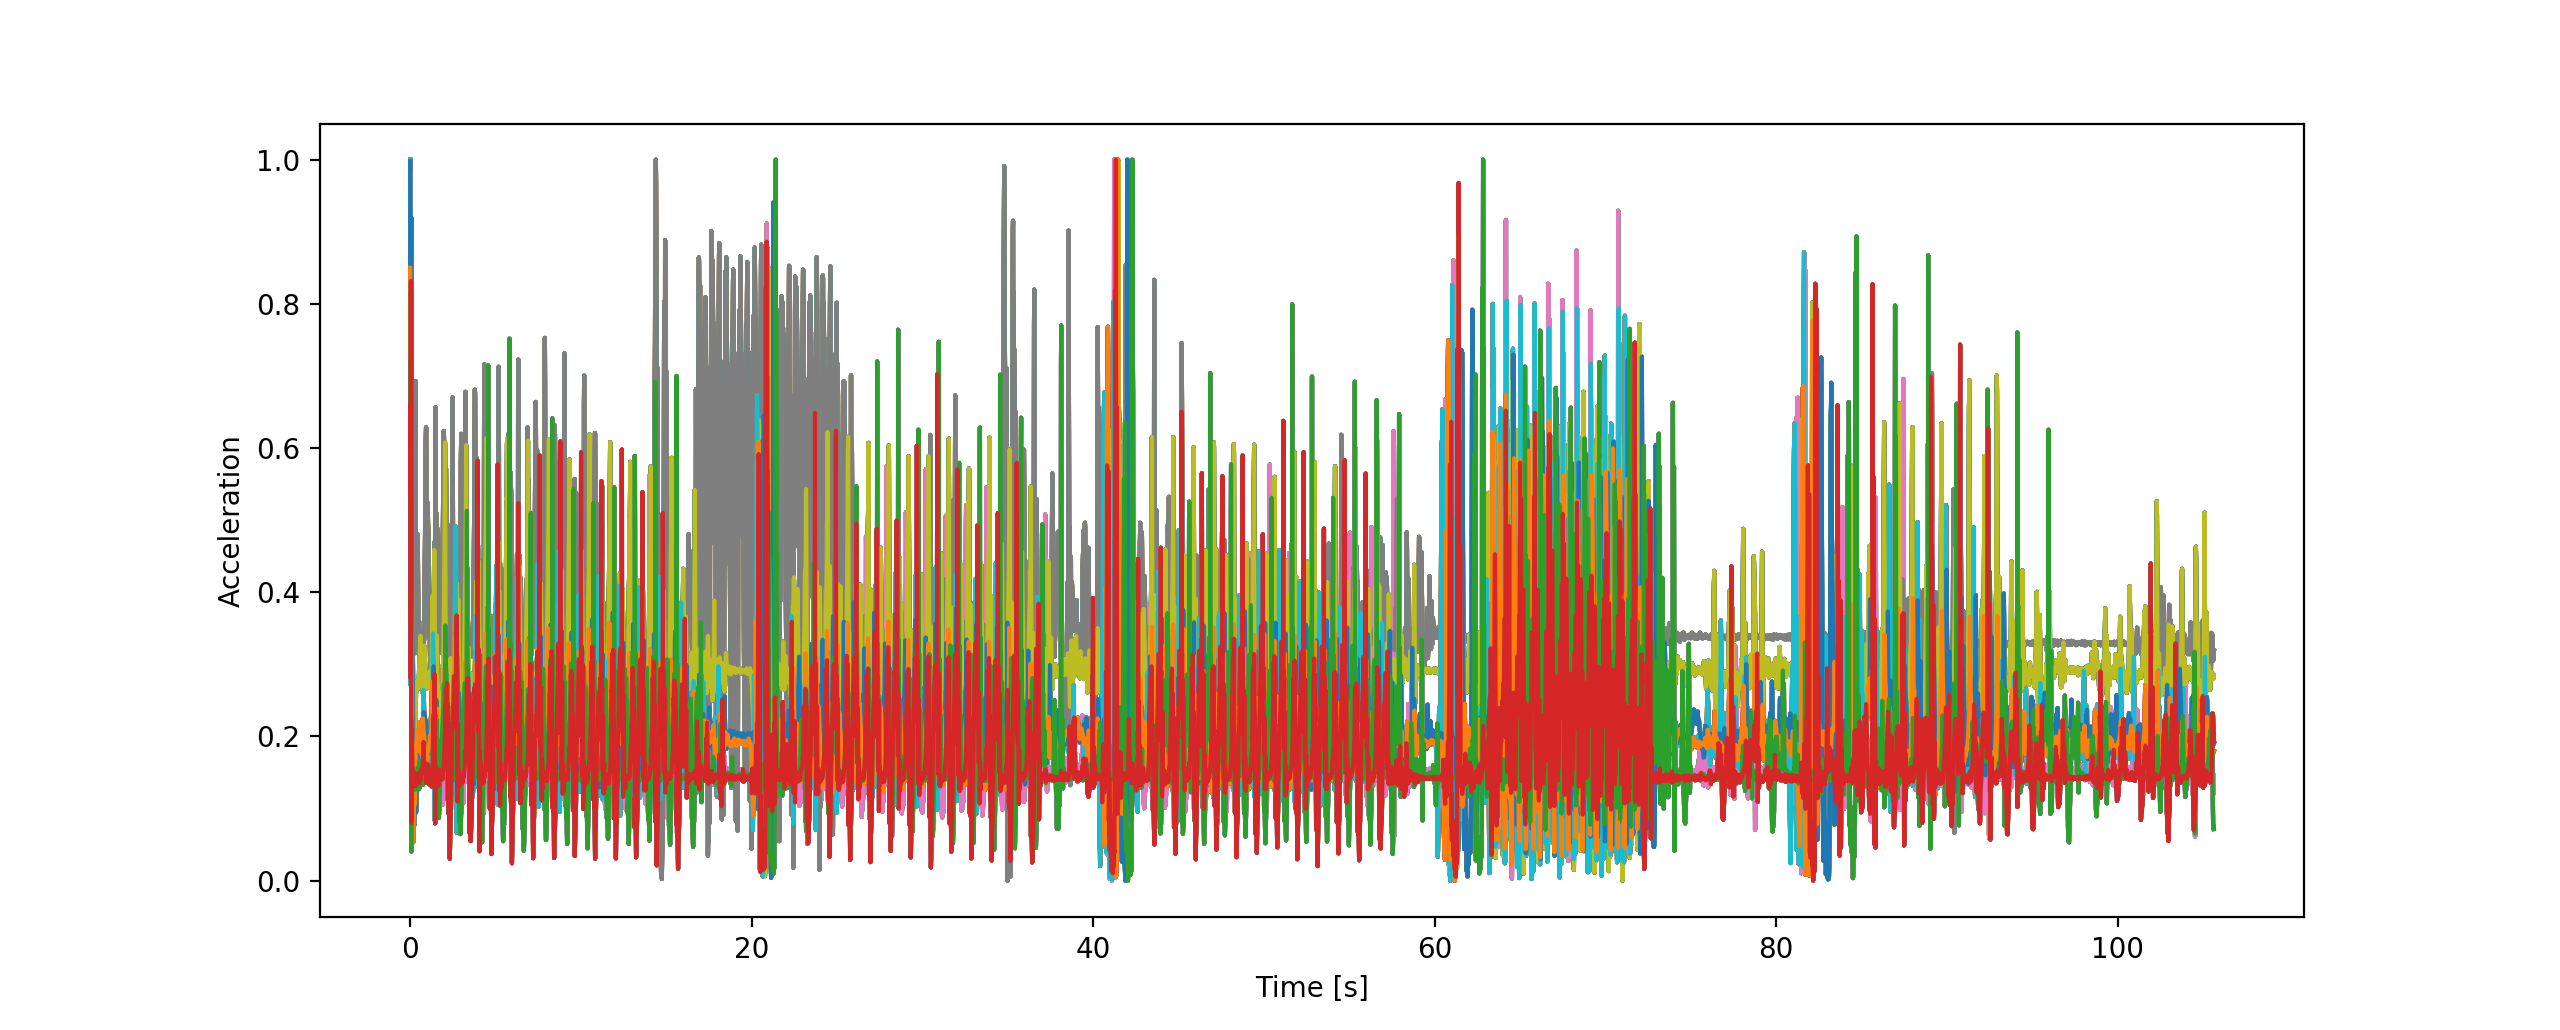
\includegraphics[width=15cm,height=8cm]
    {include/figure/AllCyc.png}
    \caption{A plot of the collected accelerometer data where the peaks represents the initilisation signals and the different colours represents the different accelerometer signals.}
    \label{fig:AllCyc}
\end{figure}

\section{Results of Pre-Evolution} \label{resultsOfPreEvolution}

\begin{figure}[htbp]
    \centering
    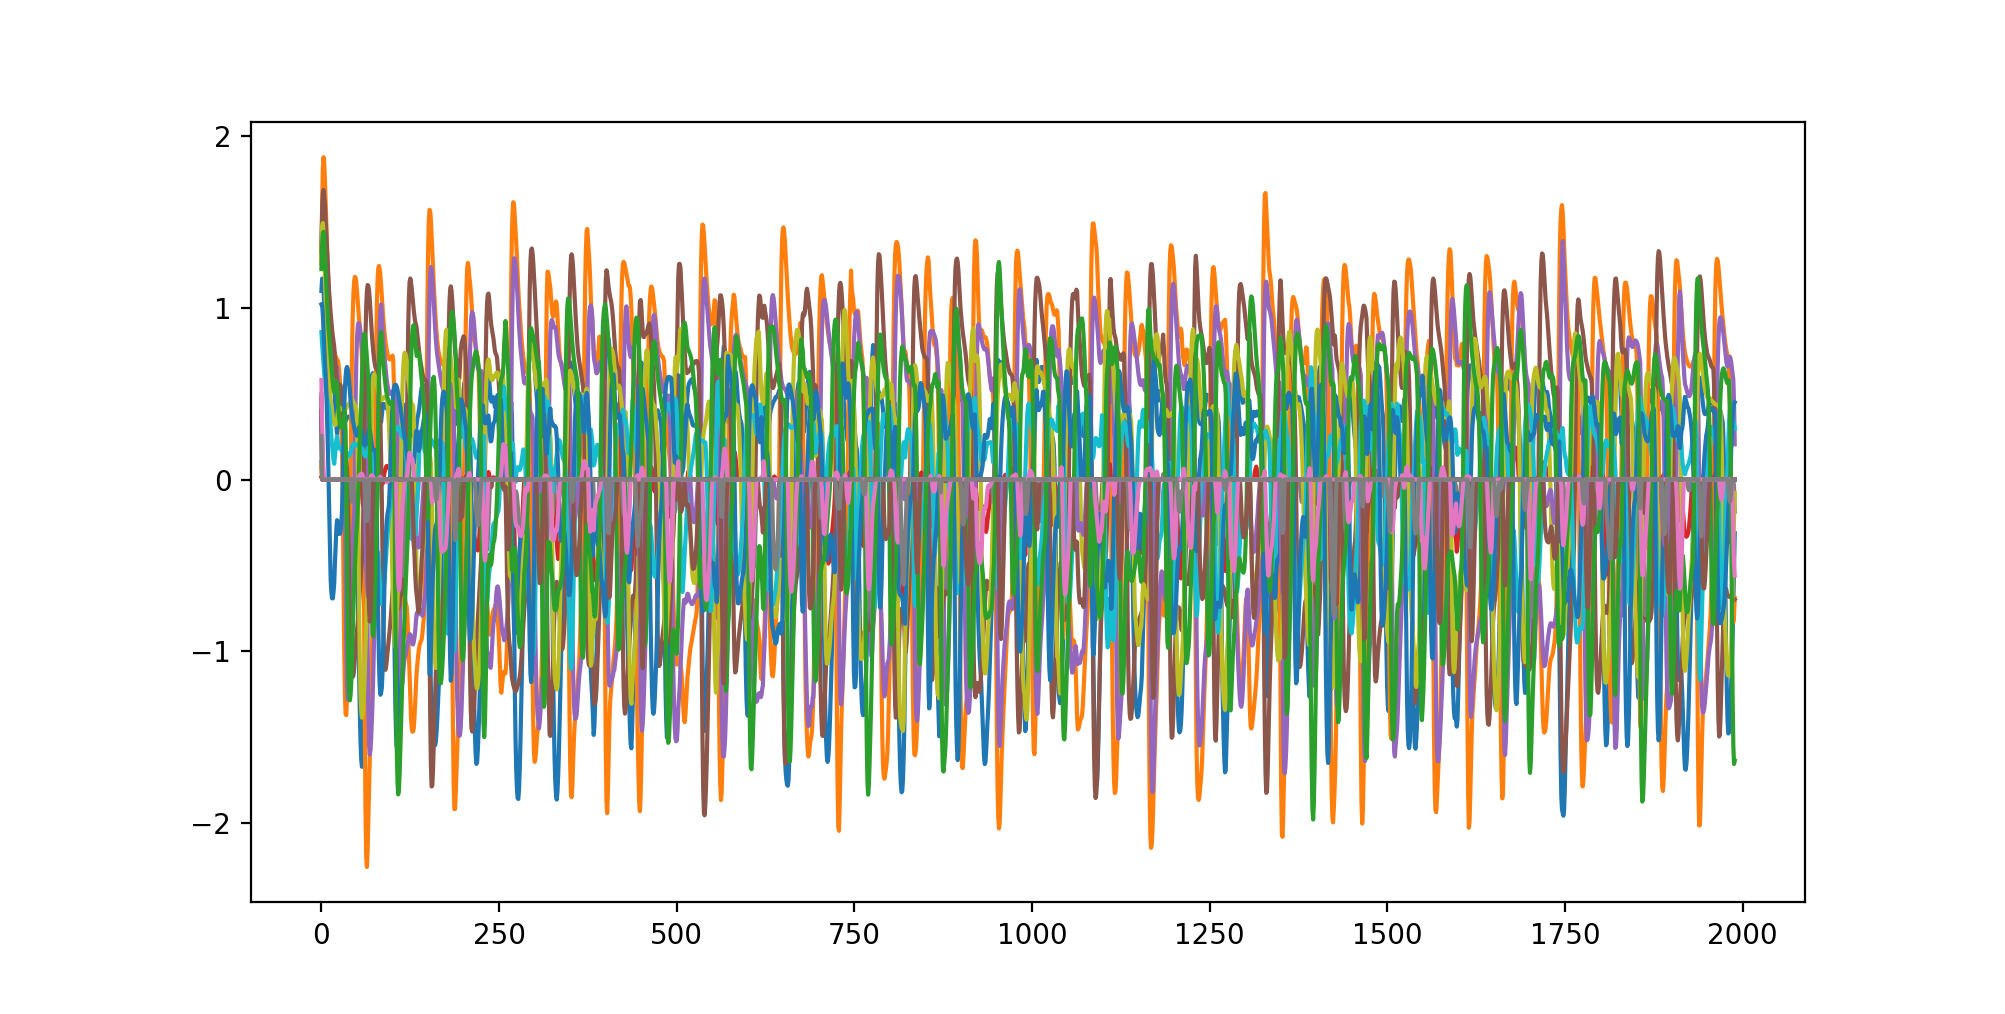
\includegraphics[width=\textwidth]{include/figure/output_500gen_w.png}
    \caption{All output signals of the best individual after 500 generations simulated. The x-axis is the simulation time, and the y-axis is the output signal represented in acceleration.}
    \label{fig:output}
\end{figure}


\begin{figure*}[t!]
    \centering
    \begin{subfigure}[b]{0.45\textwidth}
        \centering
        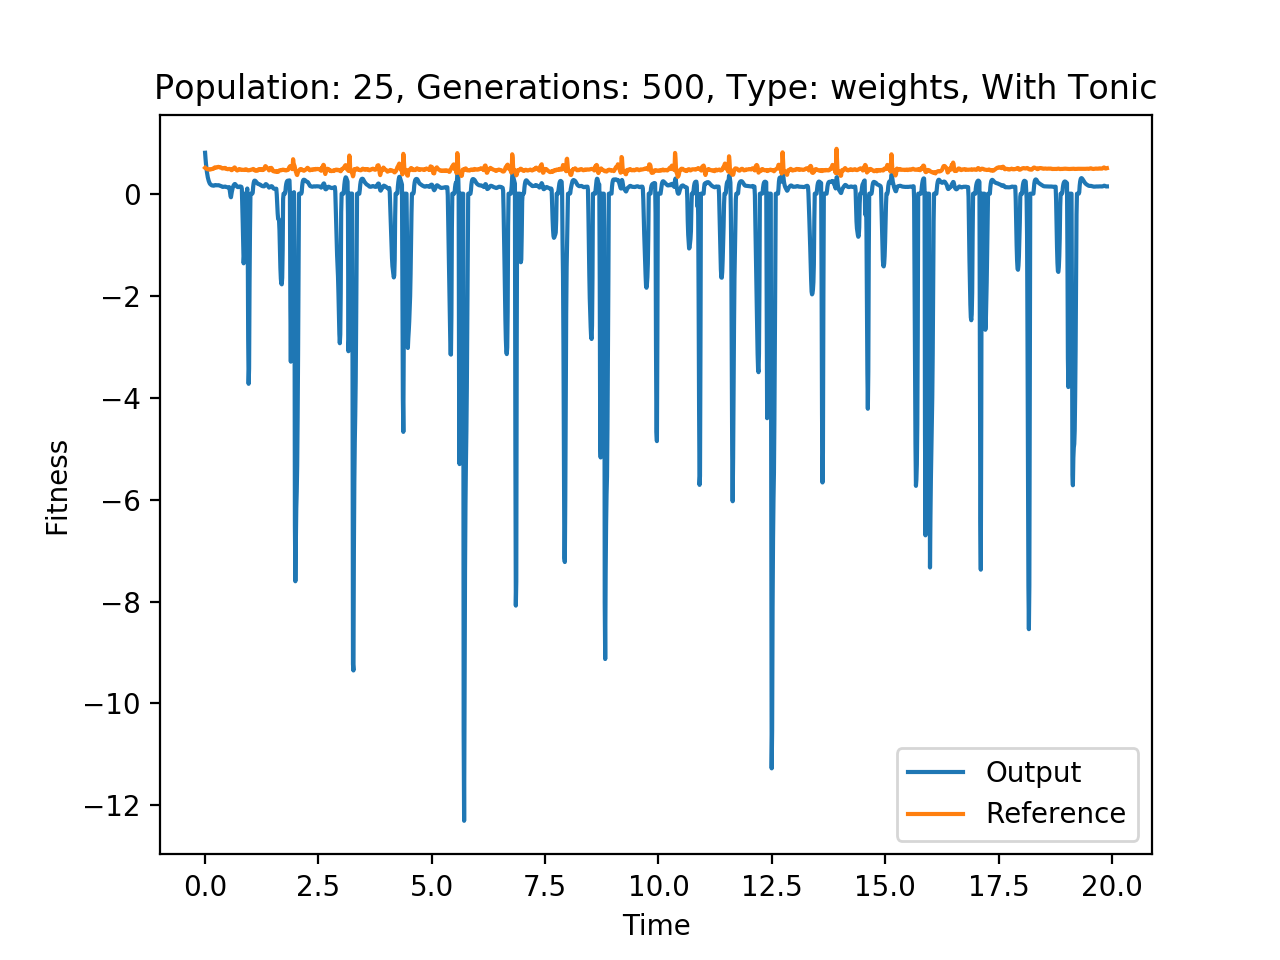
\includegraphics[width=0.95\textwidth]{include/figure/output_pop25_gen500_type0_with.png}
        \caption{Original version}
    \end{subfigure}
    ~ 
    \begin{subfigure}[b]{0.45\textwidth}
        \centering
        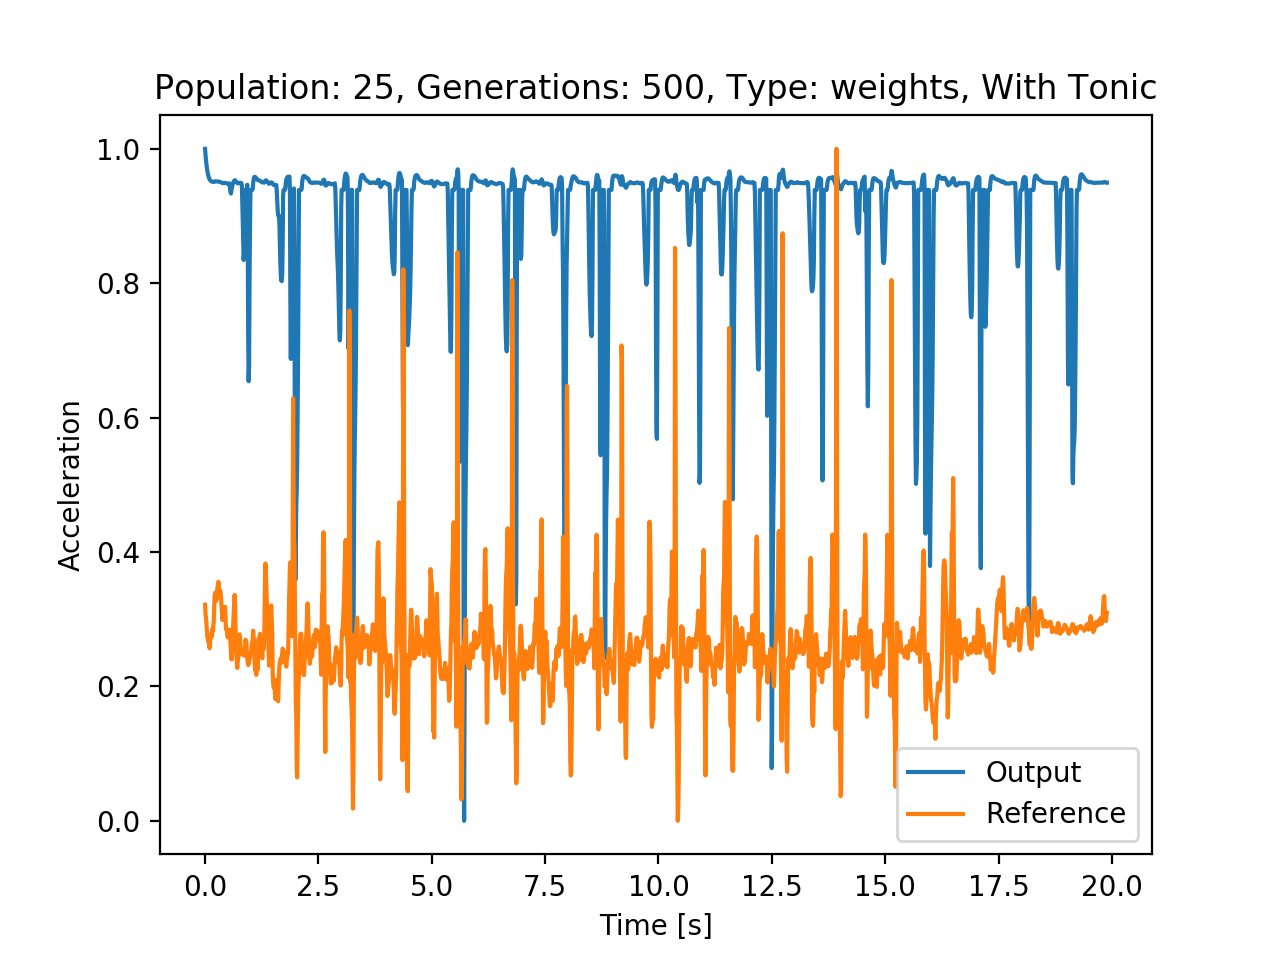
\includegraphics[width=0.95\textwidth]{include/figure/output_pop25_gen500_type0_with_normalised.png}
        \caption{Normalised version}
    \end{subfigure}%
    \caption{Output signals of the CPG network.}
    \label{fig:result_2}
\end{figure*}
\end{document}

\begin{comment} In general with generic algorithms, a large portion of their performance depent on the quality of the fitness function. Further constraints could have been made on the fitness function, for instance constraining the output signals of the left and right joints of the same type (e.g. left and right hip) to be mirror eachother, to create a more realistic oscillatory symmetric movement.\end{comment}
